\documentclass[journal]{IEEEtran}

% Add more packages here that you need!
\usepackage{graphicx} 
\usepackage[margin=1in]{geometry} 
\usepackage{amsmath,amsthm,amssymb}
\usepackage[noend]{algpseudocode}
\usepackage{amsfonts}
\usepackage{amsmath}
\usepackage{float}
\usepackage{mathrsfs}
\usepackage{booktabs}
\usepackage[nodisplayskipstretch]{setspace}
\usepackage{hyperref}
\setstretch{1}
\setlength{\abovedisplayskip}{0em}
\setlength{\belowdisplayskip}{0.5em}
\makeatletter
\def\BState{\State\hskip-\ALG@thistlm}
\makeatother

\usepackage{color}
\usepackage{pdfpages}
\usepackage{subcaption}
\usepackage[font=small,labelfont=bf]{caption}


\newcommand{\link}[2]{\href{#1}{\color{blue} \underline{\smash{#2}}}}


\begin{document}
\pagenumbering{arabic}
\def\arraystretch{1.2}

\title{Mobile Robotics WN2020 Team 4 Report}
\author{Chao Chen, Sumukha Udupa, Yutian Han, Gregory Meyer \\ \{\link{mailto:joecc@umich.edu}{joecc},\link{mailto:sudupa@umich.edu}{sudupa},\link{mailto:kevinyut@umich.edu}{kevinyut},\link{mailto:gregjm@umich.edu}{gregjm}\}@umich.edu}
\date{2020-04-30}

\maketitle
\begin{abstract}
Our project compares the results of localizing a robot with three methods: incremental SLAM with loop closure, trajectory smoothing, and filtering with a Left Invariant Extended Kalman Filter (LI-EKF). This report evaluates each of them based on the pose error accumulated over a trajectory from the North Campus Long Term (NCLT)\cite{nclt} dataset.
\end{abstract}

\IEEEpeerreviewmaketitle

\section{Introduction}\label{sec:intro}
The methods we implemented were tested against the NCLT dataset, which consists of data collected by a Segway robot on the University of Michigan's North Campus. The Segway is fitted with a spherical camera, 3D lidar, two planar lidars, a 9-DoF inertial measurement unit (IMU), a single-axis fiber optic gyro (FOG), a consumer grade GPS receiver, and a real-time kinematic (RTK) GPS receiver. The NCLT dataset consists of 27 discrete runs, each approximately an hour and a half long. The robot and the map used are shown in Figure \ref{fig:Robot}. All evaluation performed was using the run collected on 2012-11-16.

\begin{figure}
    \centering
    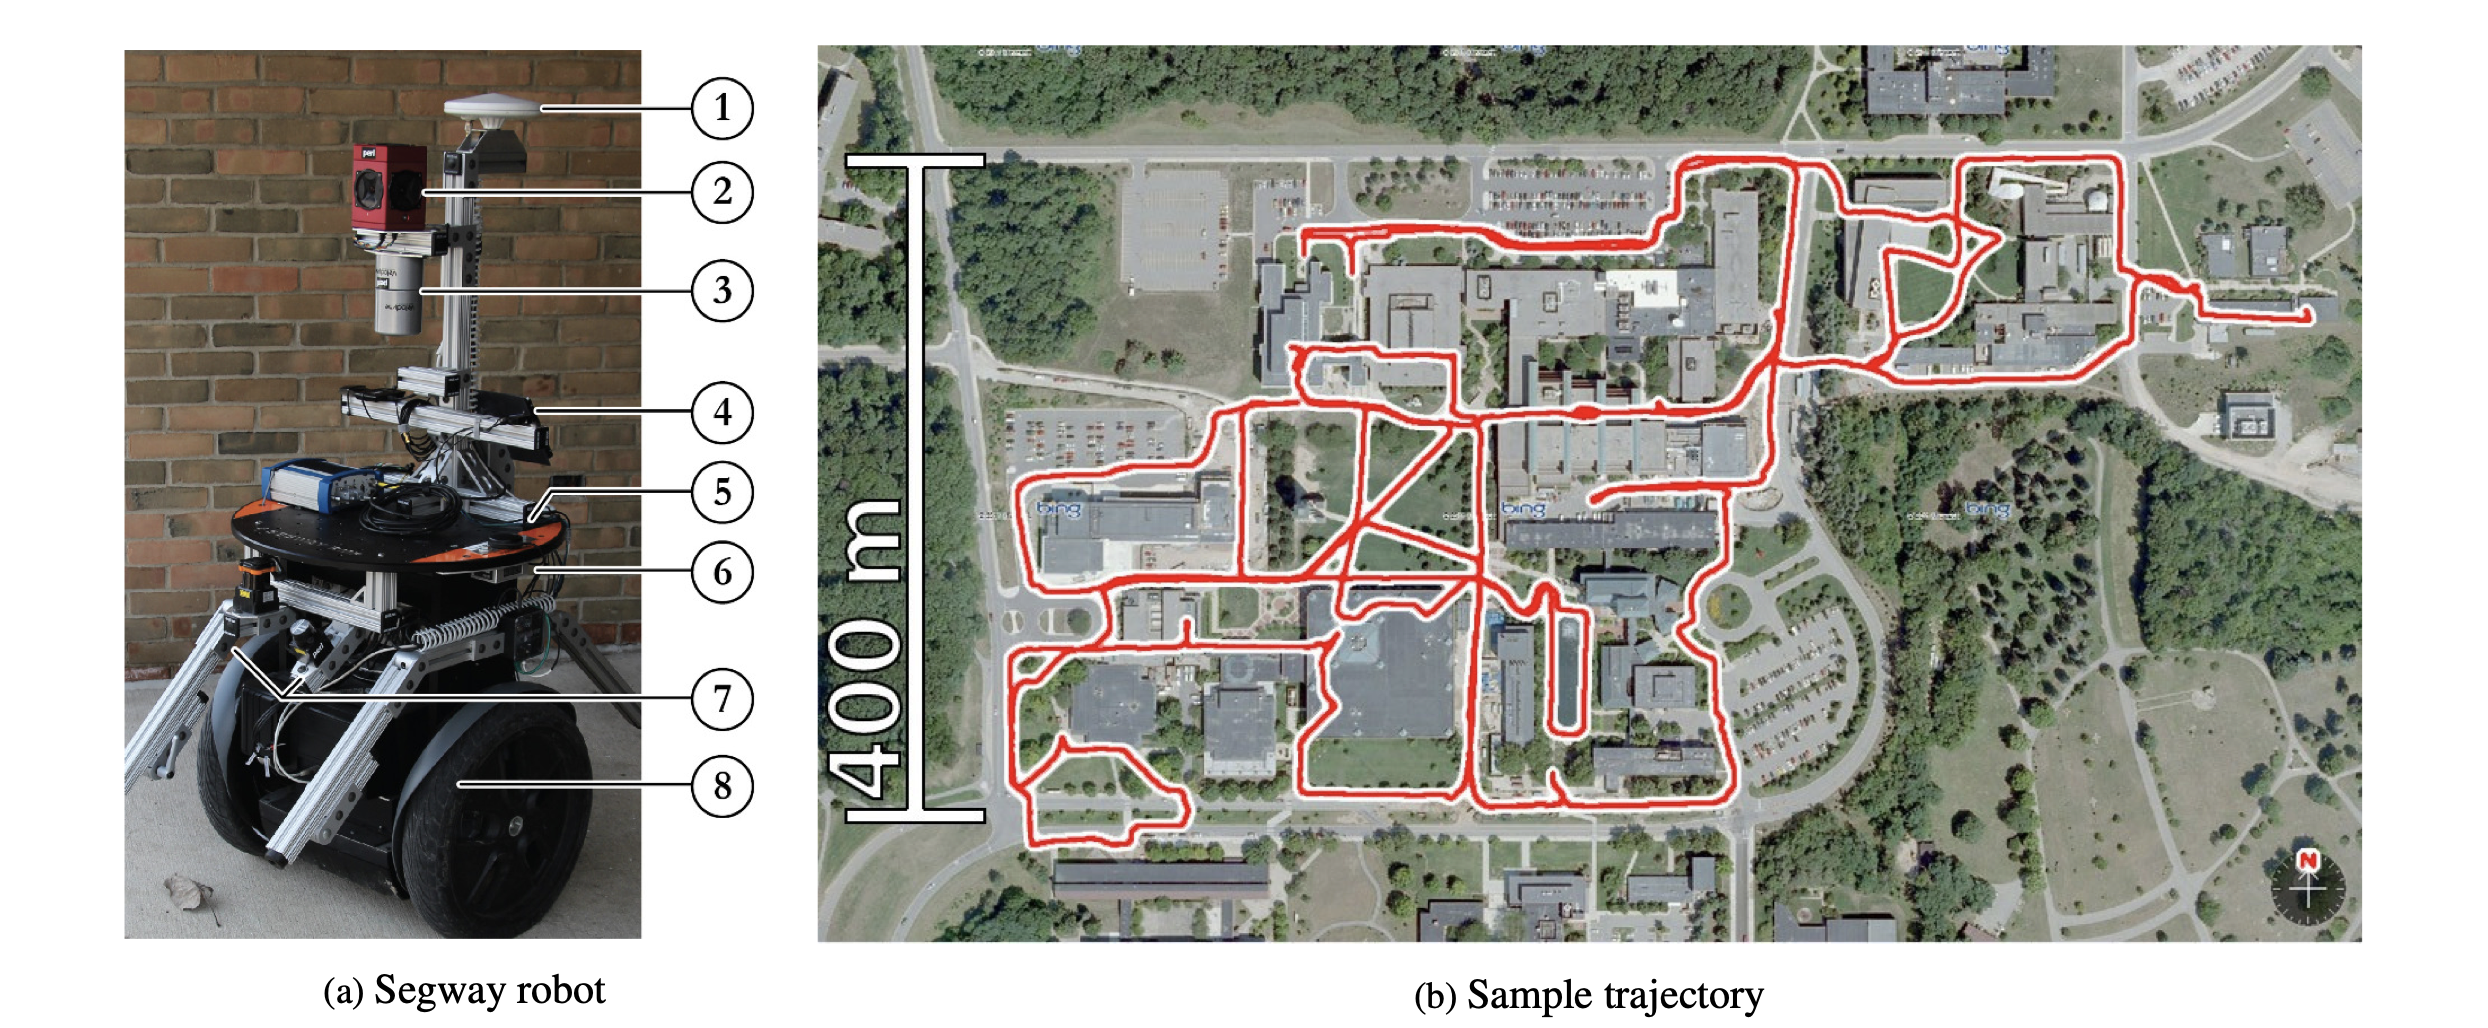
\includegraphics[width=1\columnwidth]{media/Robot_intro.png}
    \caption{The Segway robotic platform used for experimental data collection from NCLT.}
    \label{fig:Robot}
\end{figure}


\section{Methodology}\label{sec:method}
\subsection{Incremental SLAM and Loop Closure}

Incremental SLAM is normally used for online applications where the robot must continually estimate its pose while it is operating. In this section, the focus is on using online incremental lidar SLAM and loop closure to optimize the trajectory of the Segway. Cartographer\cite{cartographer}, an open-source library, is used to provide the base implementation for online SLAM. The implementation fuses measurements from the HDL-32E, wheel odometry, IMU, and FOG.

\subsubsection{Cartographer Overview}

Cartographer performs local SLAM via scan-to-submap matching with the Ceres\cite{ceres} nonlinear optimization library. Lidar scans are accumulated into fixed-size submaps (voxel grids in 3D or pixel grids in 2D), where new scans are inserted into the submap by minimizing the cost of introducing that scan into the submap, normalized by the magnitude of translation and rotation. The initial guess for the scan's alignment into the submap is formed by integrating odometry and IMU measurements observed since the last lidar measurement. Once a submap has accumulated a certain number of scans, it is marked as finalized and inserted into a pose graph for global SLAM. A subset of lidar measurements are also inserted directly into the pose graph.

Global SLAM is accomplished by optimizing the sparse pose graph of lidar measurements and submaps to jointly determine the pose of all lidar measurements and submaps. A lidar measurement should have a suitably high score when scan matched with a nearby submap, the relative pose between the two is added to the optimization problem. Adding constraints to ensure the alignment of submaps and lidar measurements increases the accuracy of the resulting trajectory in the case of loop closures.

Notably, Cartographer does not incorporate or estimate covariances for the output trajectory.

\subsubsection{Data Sources}

The input is fused from the Velodyne HDL-32E lidar, wheel odometry, the IMU, and the FOG. The raw Velodyne packets were transformed into a coordinate frame colocated with the original frame, but rotated so that its x-, y-, and z-axes are aligned with that of the IMU. We used the fused output of an Extended Kalman Filter which took the wheel odometry, IMU, and FOG as inputs as our odometry input to Cartographer; this output was provided by the authors of the NCLT dataset. Also, raw IMU data is directly inputted to Cartographer to increase the accuracy of its initial guess for scan-to-scan rotational alignment.

% TODO: test with the InEKF filtered input instead?

\subsubsection{Dimensionality}

Cartographer is tested in both 2D and 3D mode. 3D mode is particularly sensitive to the accuracy of the coordinate frame transform between the IMU and the lidar, while the flattening behavior used for 2D mode permits more leeway in the alignment between the two. The authors of the NCLT dataset have included an accurate transform between the two coordinate frames, computed by jointly optimizing for the SLAM problem and the alignment of the lidar. Applications, where the angular error of the IMU-to-lidar coordinate frame transform is on the magnitude of a degree or more are likely to see a poor performance if they attempt to use Cartographer for 3D SLAM.

\subsubsection{Local SLAM Tuning}

Local SLAM is tuned primarily by modifying the cost of modifying linear and rotational translation from the initial guess. Our group tested several combinations of increasing and decreasing the linear and rotational weight relative to the default values.

\subsubsection{Implementation}

this part of the project is implemented in C++17, using Cartographer's C++ interface. Arbitrary runs from the NCLT dataset can be provided as input, and output is emitted as a CSV file in the same format as the ground truth data provided by the NCLT dataset. As Cartographer does not support covariance estimation for the optimized trajectory, no covariance is output. Odometry data may optionally be provided; users should take care to use the 100Hz odometry computed relative to the initial pose of the robot, not the odometry computed relative to the last odometric pose. CMake 3.11 or newer is used as a metabuild system. Additionally, Cartographer, Boost 1.58 or newer (including the iostreams component), and Eigen 3 are build-time dependencies.

A Python wrapper script is provided with the implementation. This script automates building and running the C++ part of the project similar to Rust's \texttt{cargo} package management utility. Further usage information can be obtained by running \texttt{python csv\_slam.py --help}. Subcommands also support the \texttt{-h,--help} option to emit help text.

\subsection{Trajectory Smoothing}
Trajectory smoothing method is normally used if the whole dataset is given as a whole. Then the path of the robot can be further optimized using this method. In this section, the focus is on the optimization capability of trajectory smoothing method.

Four different sources of data are used and processed as the prediction and measurement including GPS data, IMU data, Odometry data, and gyro data. In the following discussion, three modifications of the data are discussed including filtering odometry data with gyro data, filting GPS data with IMU data, and filtering odometry data is used as the prediction step and modified GPS data is used for correction measurement.

\subsubsection{Gyrodometry}
Before processing the datasets, ``gyrodometry" method is introduced in \cite{borenstein1996gyrodometry} referenced to determine the fused yaw angle change \(\Delta \psi\). One simple experiment is implemented to test on this method. The  bot  was  moved  along  a  groundtruth trajectory (Fig. \ref{fig:odometry_traj}), and the raw sensing data \(n_R\), \(n_L\), and \(\dot{\psi}_{IMU}\) were logged. \(R_R\), \(R_L\), and \(b\) were provided in the parameter sheet.

Based on the data measured on the robot, the yaw angle and angular velocity from pure wheel odometry and IMU, as well as their difference are shown in Fig. \ref{fig:odometry_angle_diff}. According to the figure, the typical range of the \(\dot{\psi}\) difference is within \(\pm\)0.5 rad/s. And the difference between \(\psi\) is generated mainly during the turning process, where the typical \(\dot{\psi}\) difference is within \(\pm\)0.3 rad/s. These show that a meaningful \(C_{\dot{\psi}}\) will be between 0-0.5 rad/s.

The gyrodometry was run on different \(C_{\dot{\psi}}\). According to the result in Fig. \ref{fig:odometry_tune}, always using yaw information from IMU leads to drift in the straight line period, while always using yaw information from wheel odometry leads to larger errors during turning. Choosing \(C_{\dot{\psi}} = 0.2\) rad/s will combine the strength of both the wheel odometry and IMU, and lead to result closer to the ground truth. Therefore, the \(C_{\dot{\psi}}\) is fixed, and the onboard result with this threshold is shown in Fig. \ref{fig:odometry_traj}.

\begin{figure}[hbt!]
    \centering
    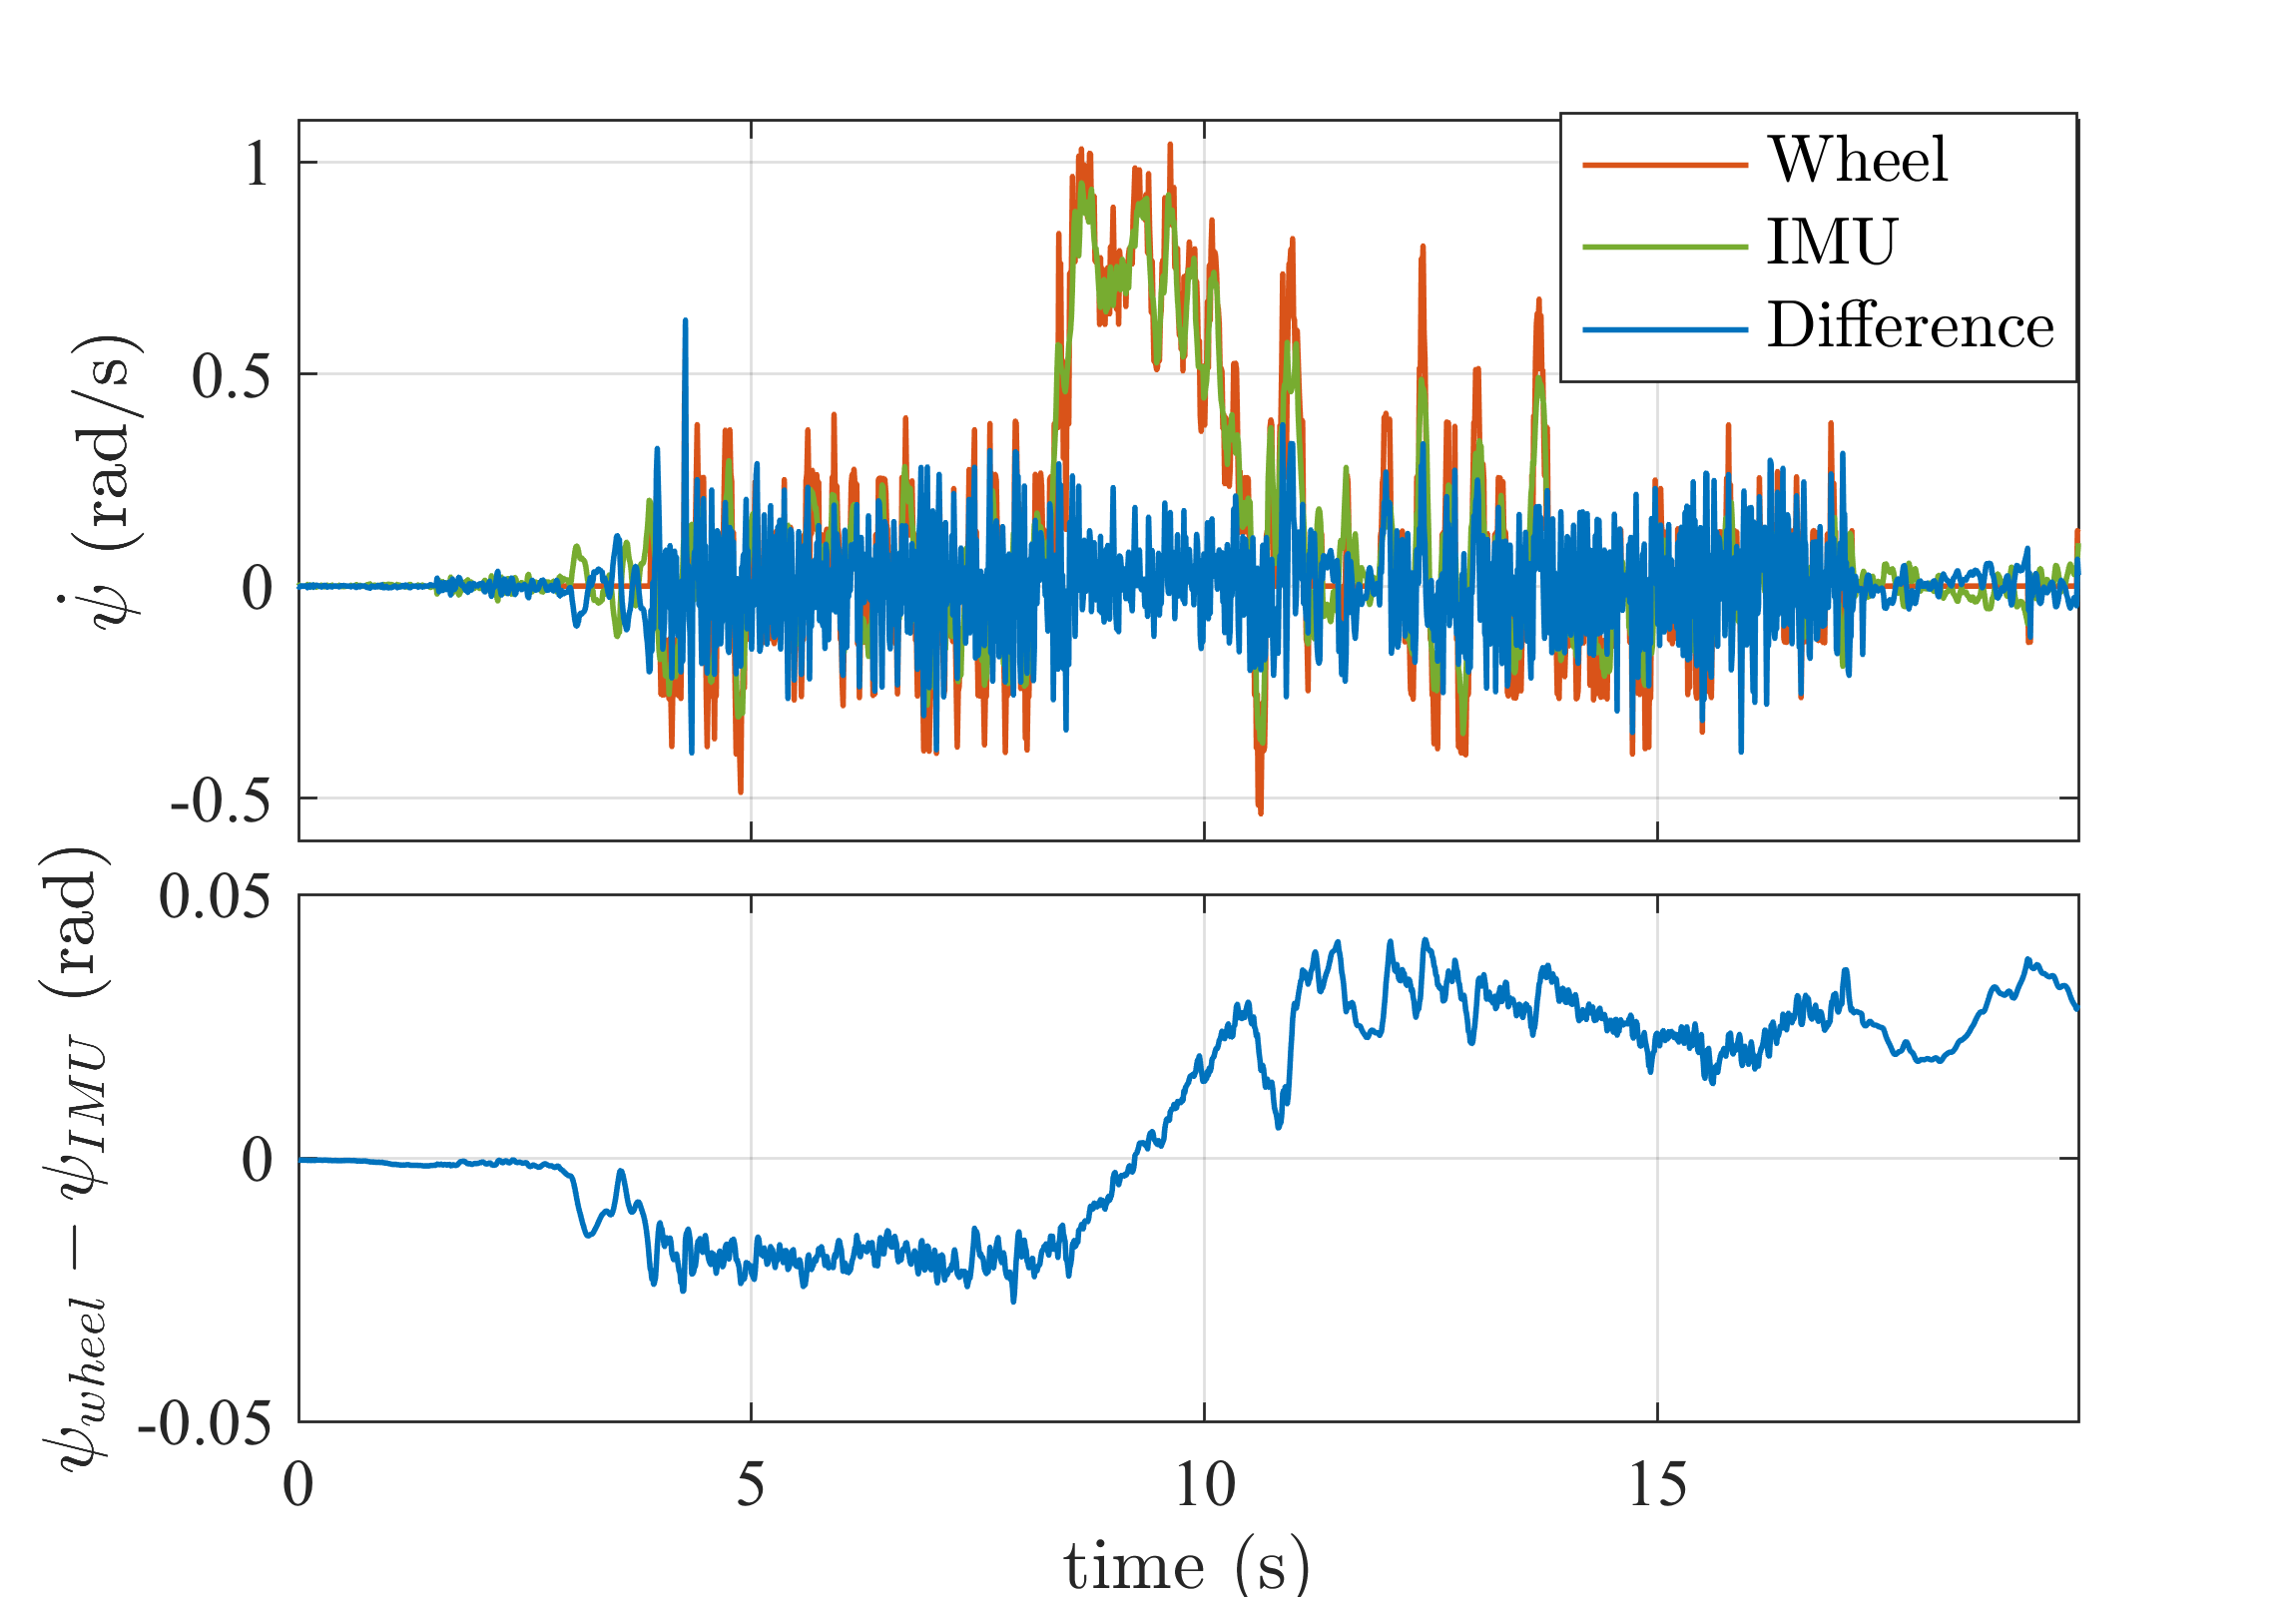
\includegraphics[width = 1.0\linewidth]{media/odometry_angle_diff.png}
    \caption{Yaw angle and angular velocity from wheel odometry and gyro.}
    \label{fig:odometry_angle_diff}
\end{figure}

\begin{figure}[hbt!]
    \centering
    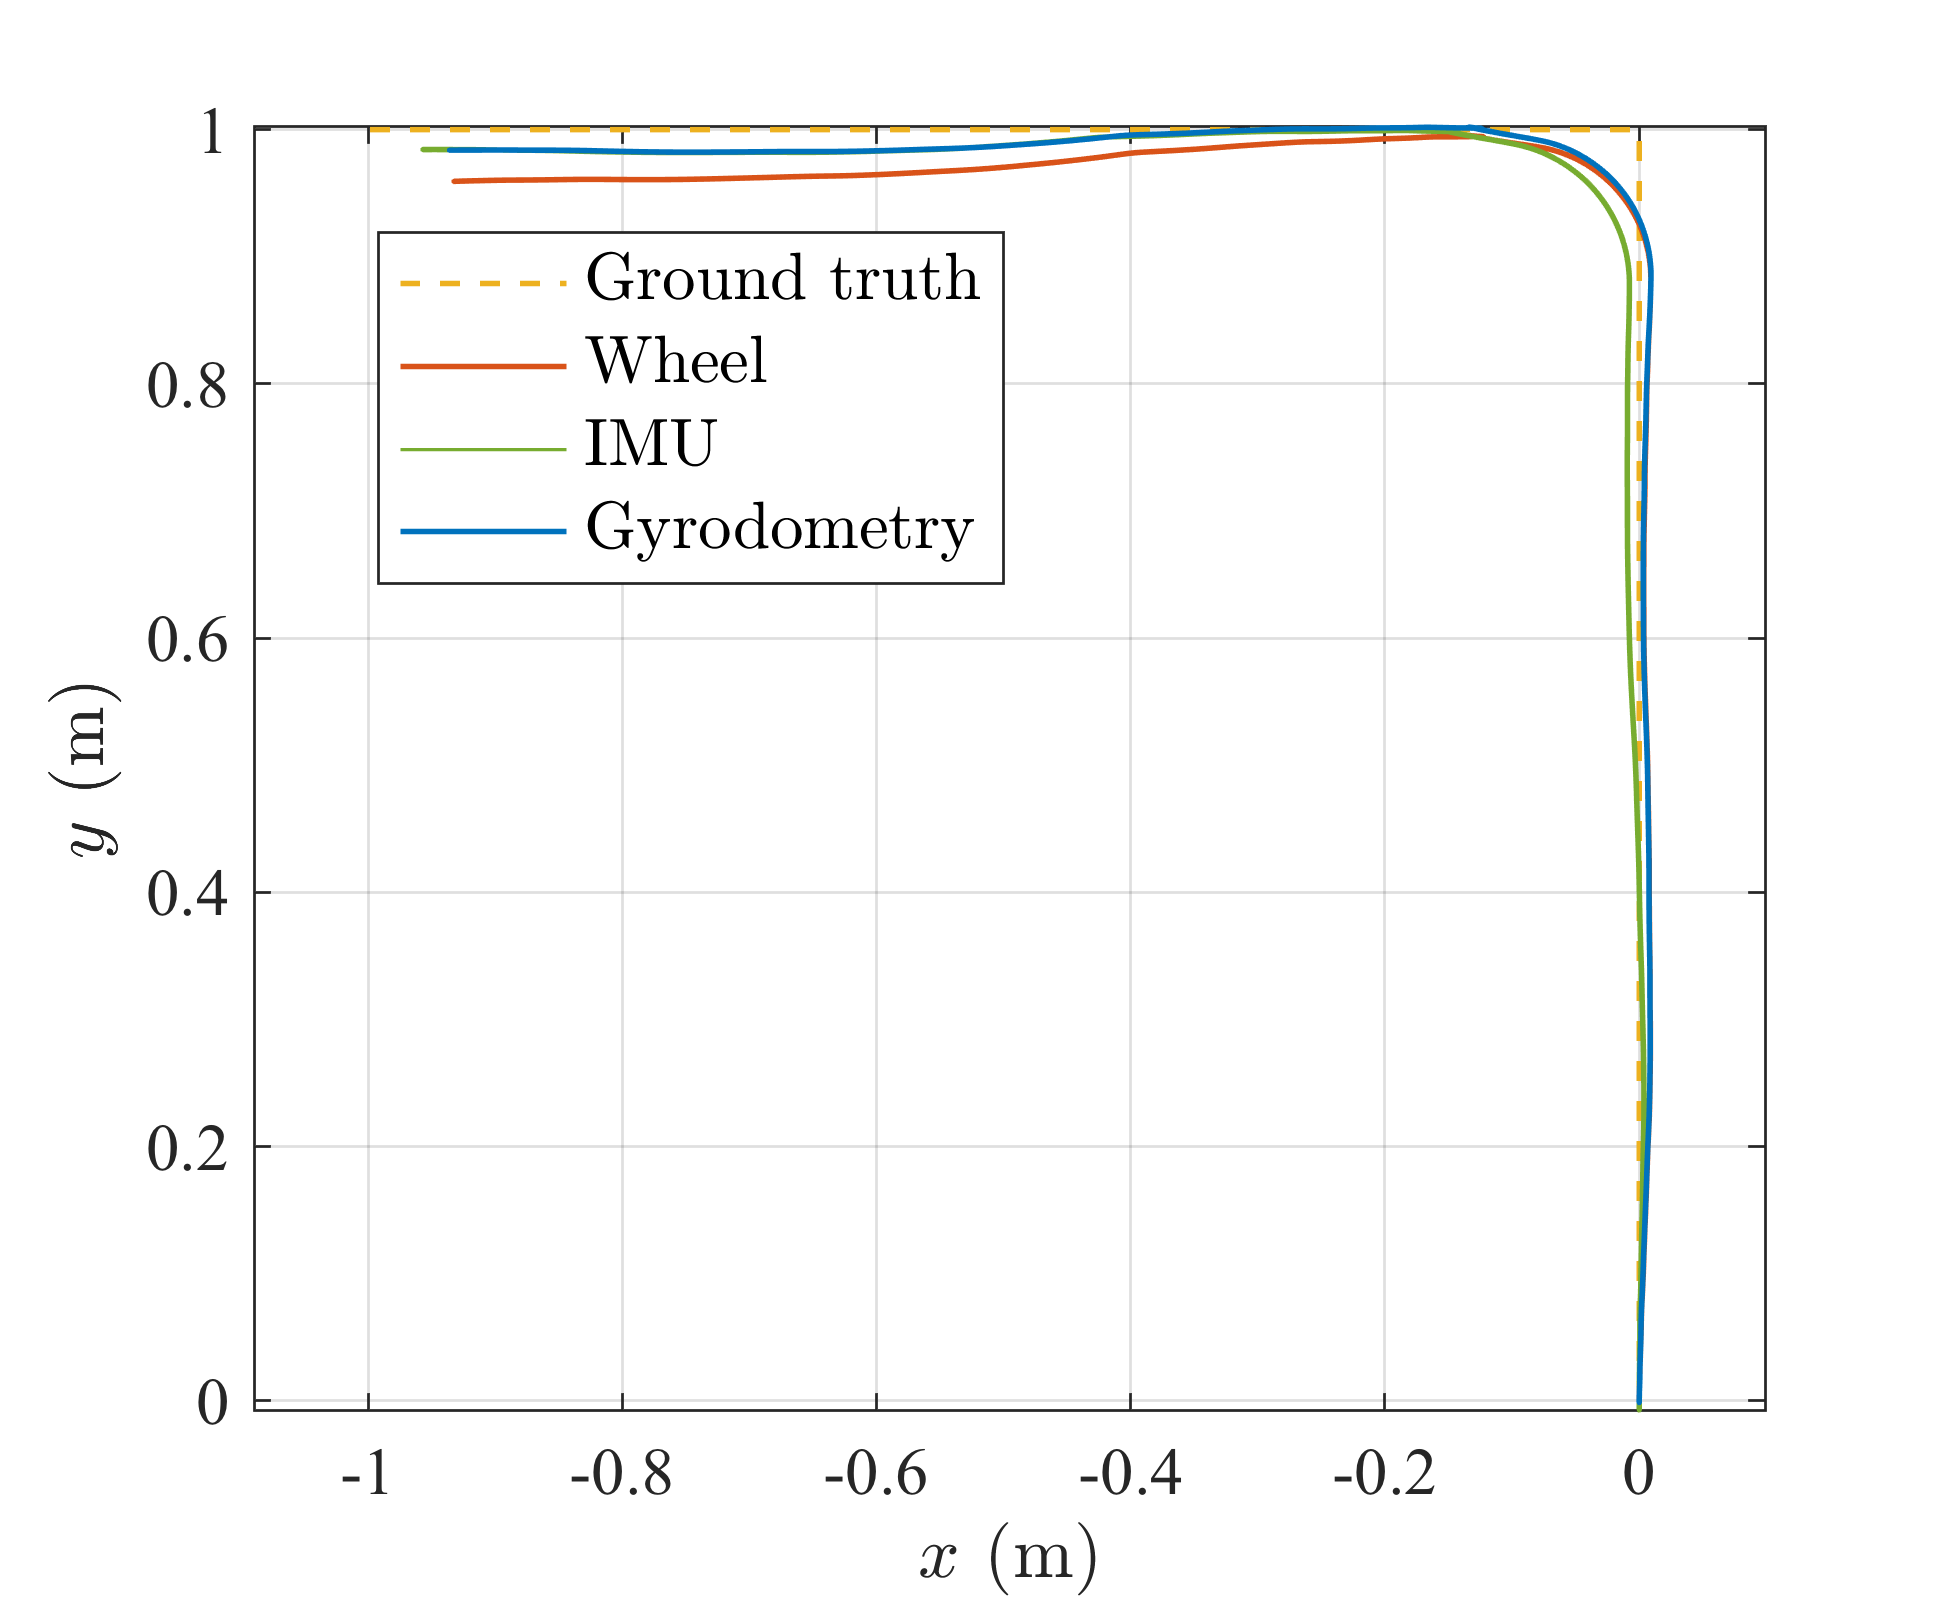
\includegraphics[width = 0.9\linewidth]{media/odometry_traj.png}
    \caption{Odometry results in different modes. The ground truth might be inaccurate during the turning process.}
    \label{fig:odometry_traj}
\end{figure}

\begin{figure}[hbt!]
    \centering
    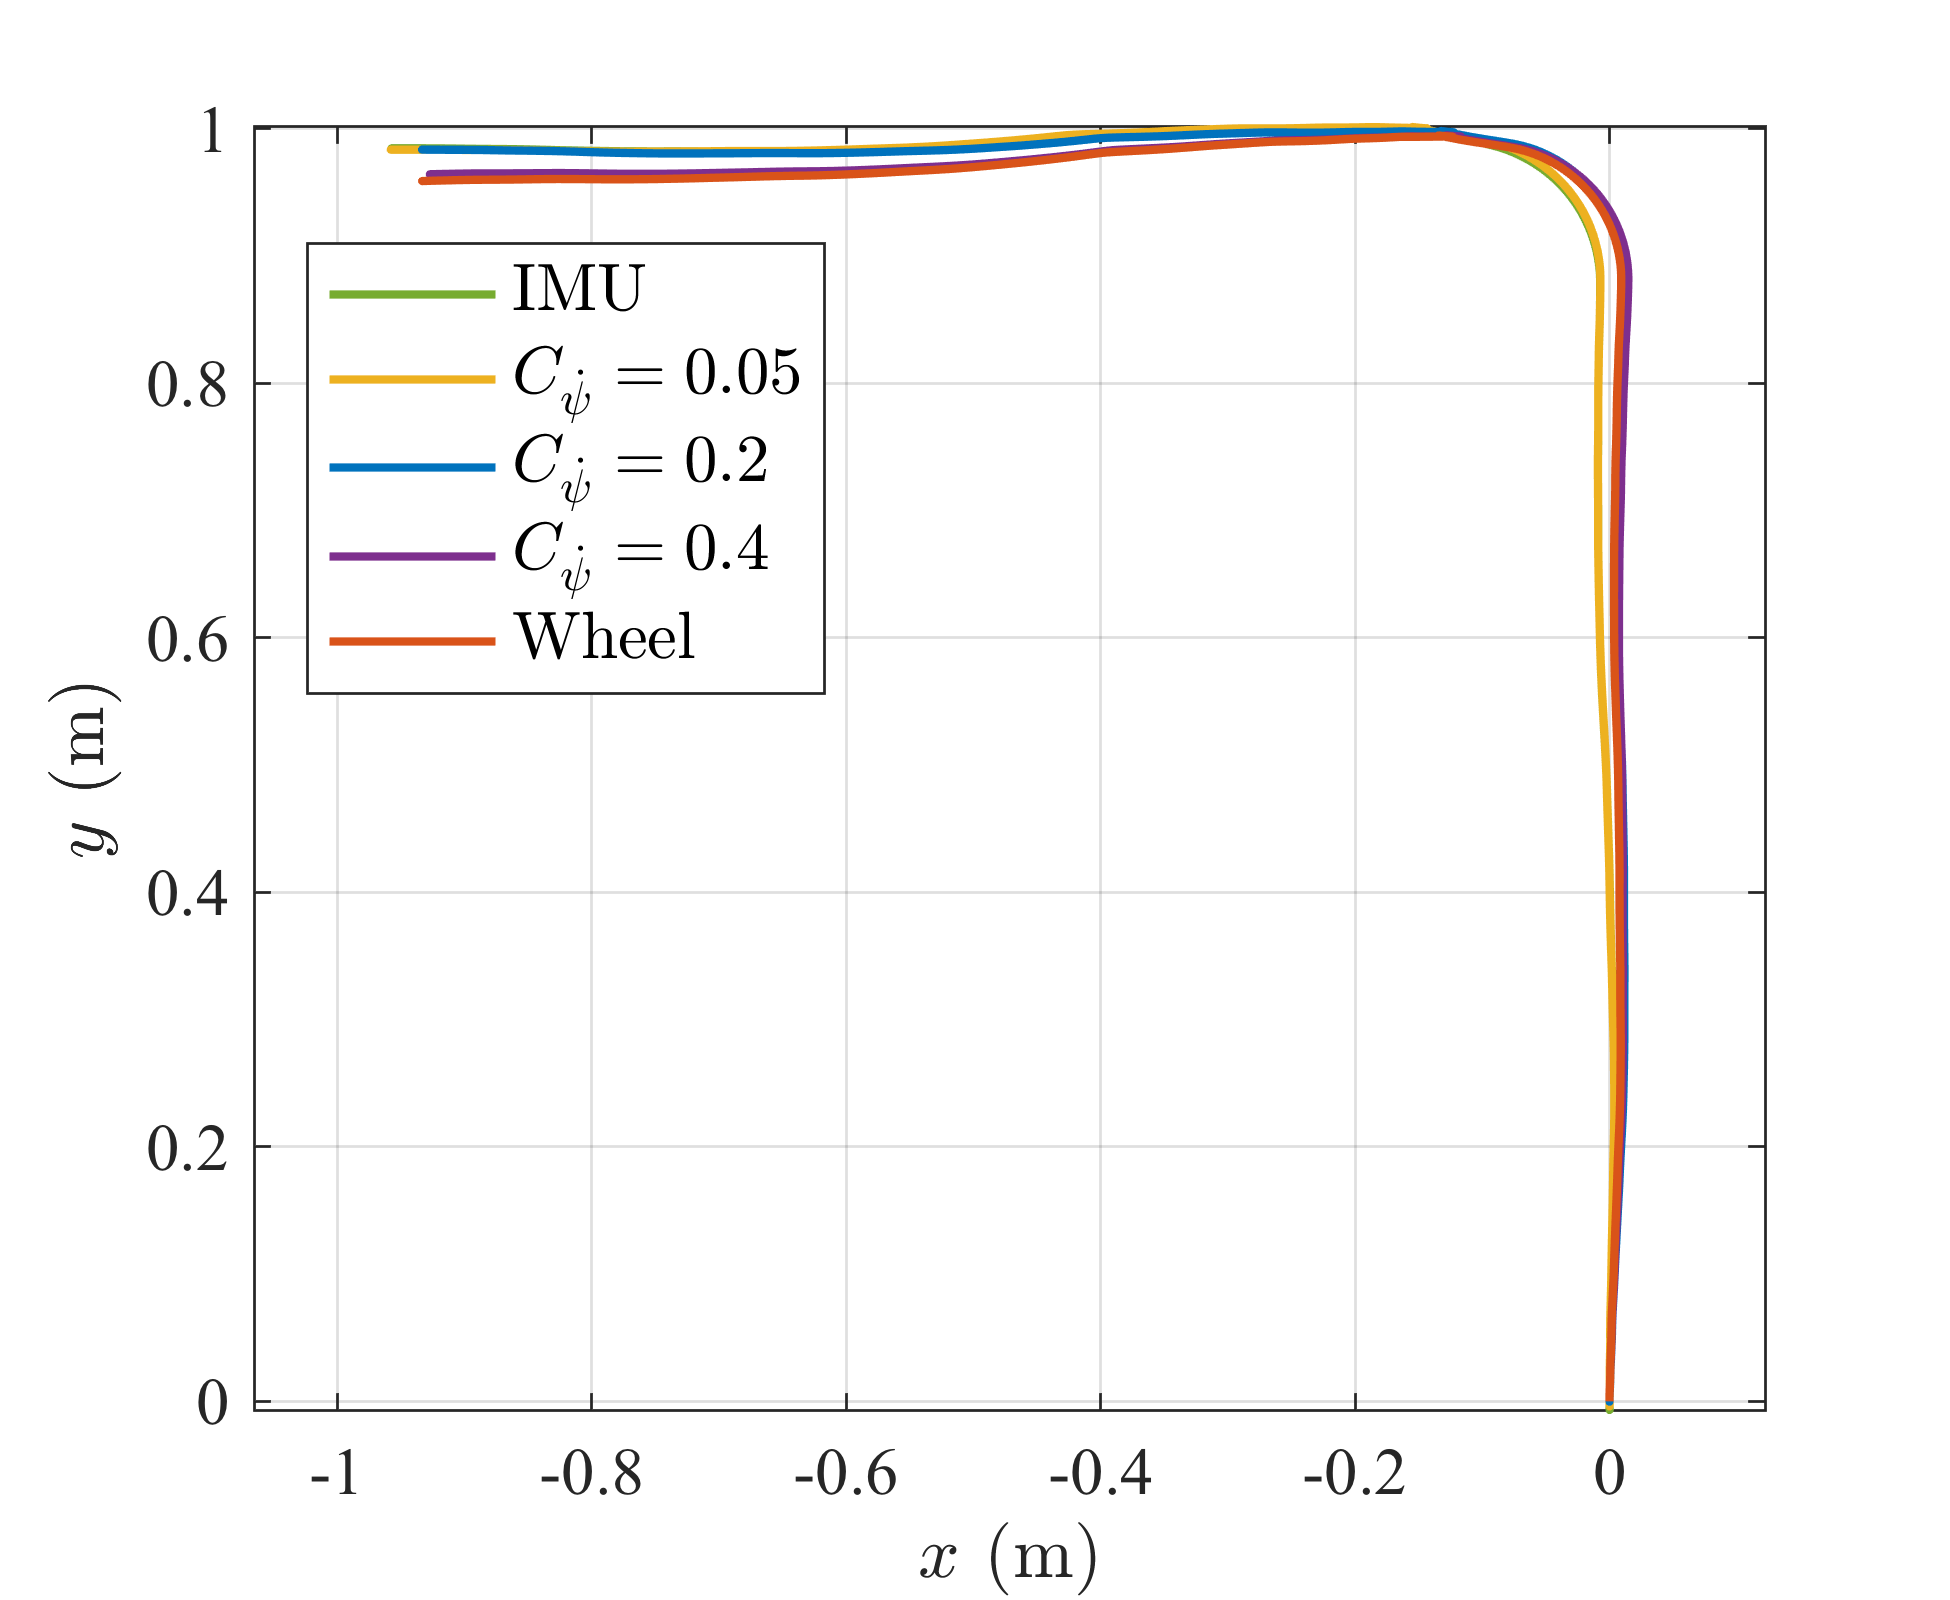
\includegraphics[width = 1.0\linewidth]{media/odometry_tune.png}
    \caption{Gyrodometry results with different \(C_{\dot{\psi}}\) (unit: rad/s) computed in MATLAB. The line of ``IMU" overlaps with ``\(C_{\dot{\psi}}\) = 0.05".}
    \label{fig:odometry_tune}
\end{figure}\label{sec:gyrodo}

\subsubsection{Odometry Fused with Gyroscope}
Now, the next step is to compute a valid set of data using odometry and gyro data. By the nature of the data type, odometry data is accurate for robot moving in a linear motion, but is inaccurate when the robot is turning due to wheel slippage. In contrast, gyro data is a good resource for estimating the turning angle, but performs poorly in linear motion. Thus, two optimization methods are given to combine odometry and gyro data.

One method labelled ``gyro-only" method in Figure \ref{fig:Gyrodometry} is to take odometry data as the prediction of the distance, whereas the FOG information \(\dot{\psi}_{\text{IMU}}\) is used for predicting the heading of the robot. 

One other optimization is the ``gyrodometry" method discribed in section.\ref{sec:gyrodo}. Besides, by experiment, the threshold value is set where \(C_{\dot{\psi}} = 0.2\)

\begin{figure}
    \centering
    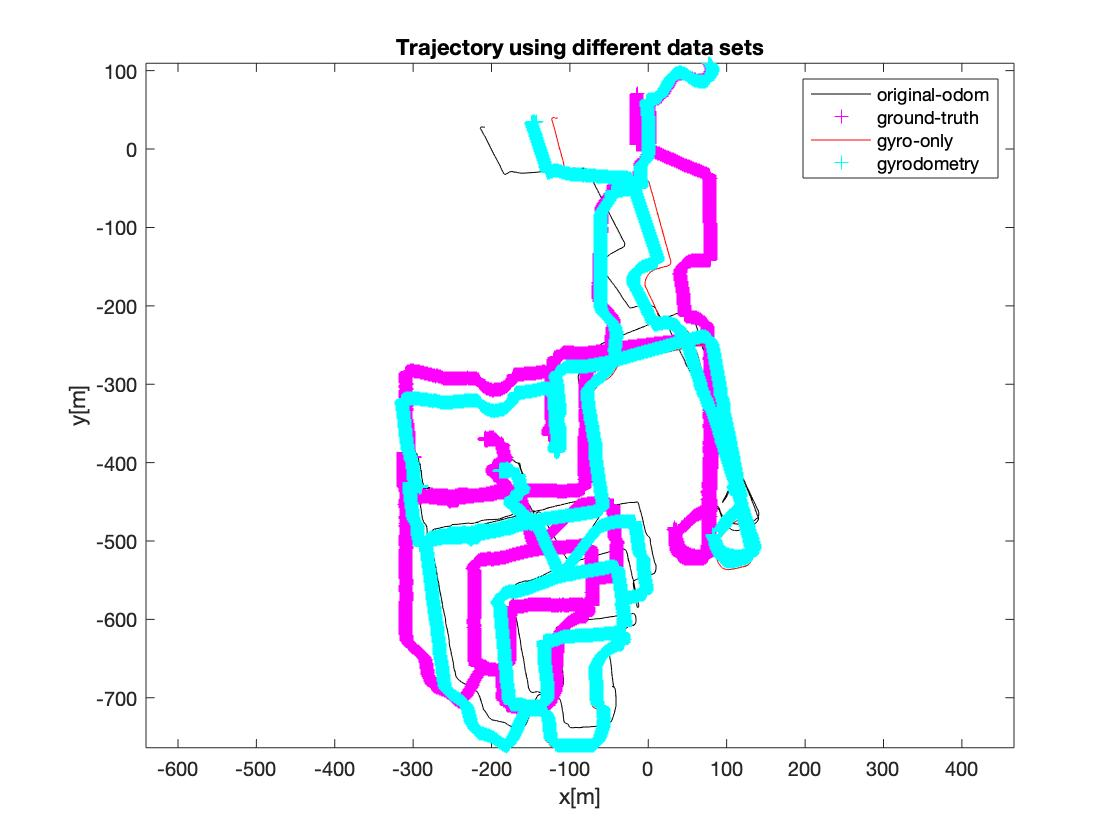
\includegraphics[width=0.8\columnwidth]{media/Gyrodometry.jpg}
    \caption{Odometry optimization using Gyrodometry method}
    \label{fig:Gyrodometry}
\end{figure}

\subsubsection{GPS Optimization using IMU}
GPS data is normally used as the measurement in the outside environment. However, by visualizing the GPS data in Figure \ref{fig:IMU-GPS}, the data contains a lot of outliers(shift in the location). Similar to previous methods where gyro data has been used for the correction of odometry data, IMU data is used to correct the orientation of the GPS data.

Notably, the method used to filter GPS data is incremental Smoothing and Mapping Using the Bayes Tree(ISAM2) describe in \cite{5979641}. After optimization, filtered GPS data is illustrate in Figure \ref{fig:filteredgps}.

\begin{figure}[hbt!]
    \centering
    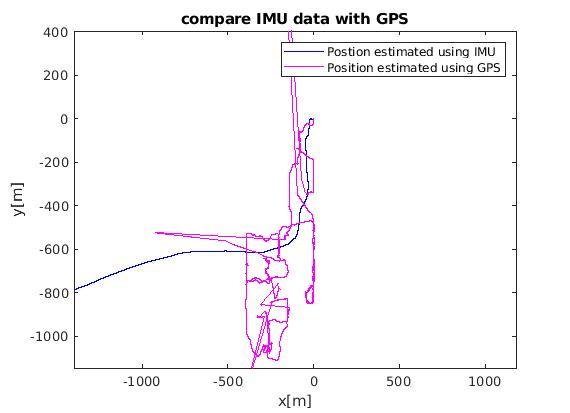
\includegraphics[width = 0.8\linewidth]{media/original-compare.jpg}
    \caption{\textit{Compare IMU data with GPS data.}}
    \label{fig:IMU-GPS}
\end{figure}

\begin{figure}[hbt!]
    \centering
    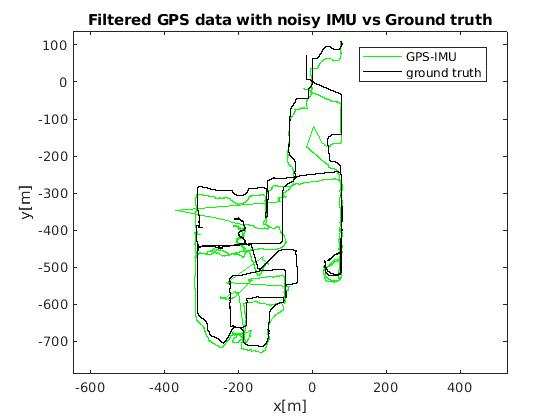
\includegraphics[width = 0.8\linewidth]{media/filteredfGPS.jpg}
    \caption{\textit{GPS data filted by IMU data.}}
    \label{fig:filteredgps}
\end{figure}

\subsubsection{Filtered Odometry with Filtered GPS}
After the filtered odometry data and filtered GPS data are obtained, in this project the last step of the trajectory smoothing is to combine these two data sets together. The method used in this case is ISAM2 in \cite{5979641}.

The steps taken are similar to those in processing GPS data. It is noticeable that the odometry obtained from Figure \ref{fig:Gyrodometry} can be a good metric for orientation, as the details of filtered odometry are similar to those of the ground truth. In contrast, the absolution position of the filtered GPS data is similar to that of the ground truth. By tuning the covariance values($\sigma$) in linear and angular direction, the final filtered graph is shown in Figure \ref{fig:Final plot}.

\begin{figure}[hbt!]
    \centering
    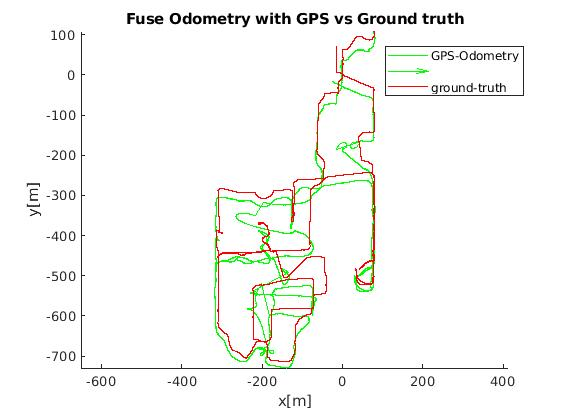
\includegraphics[width = 0.8\linewidth]{media/GPS+Odometry3.jpg}
    \caption{\textit{Compare filtered data with ground truth.}}
    \label{fig:Final plot}
\end{figure}

\subsection{Left Invariant Extended Kalman Filter}


The theory of invariant observer design, based on the estimation error being invariant under the action of a matrix Lie Group, has recently been developed to Invariant EKF, which is applied to simultaneous localization and mapping in \cite{hartley2018contact}. This section derives a Left Invariant EKF to estimate the pose of the robot in the world frame using IMU and GPS measurements. The state is modelled as:

\begin{equation}
    X_{k} = 
    \begin{bmatrix}
    R_{k} & v_{k} & p_{k} \\
    0 & 1 & 0 \\
    0 & 0 & 1
    \end{bmatrix}
\end{equation}

where $R_{k} \in SO(3)$ is the orientation, $v_{k} \in \mathbb{R}^3$ is the linear velocity, and $p_{k} \in \mathbb{R}^3$ is the global position. IMU measurements are used for prediction and GPS measurements are used for correction.

In prediction, the angular acceleration ($w_{k} \in \mathbb{R}^3$) and linear acceleration $a_{k} \mathbb{R}^3$ obtained from the IMU are utilized as input to propagate the state mean using the following equations:

\begin{equation}
    R_{k+1}=R_{k}exp(\overline{\omega_{k}}\delta t)
\end{equation}

\begin{equation}
    v_{k+1}=v_{k}+R_{k}(\overline{\omega_{k}}\delta t)\overline{a_{k}}\delta t+g \delta t
\end{equation}

\begin{equation}
    p_{k+1}=p_{k}+v_{k}+R_{k}(\overline{\omega_{k}}\delta t)\overline{a_{k}}\delta t^{2}+(1/2)g \delta t
\end{equation}

The dynamics above does not consider the in-run bias in the accelerometer, given the fact that only $\pm$0.04 mg bias exists. In order to propagate the covariance, the adjoint operator is obtained as follows:

\begin{equation}
    Ad = 
    \begin{bmatrix}
    R & 0 & 0   \\
    (v)_{\times}R & R & 0  \\
    (p)_{\times}R & 0 & R 
    \end{bmatrix}
\end{equation}

where $()_{\times}$ denotes a $3 \times 3$ skew-symmetric matrix. 
The left-invariant error dynamics depend on the IMU inputs, which are assumed to be constant (following a zero-order hold) between $t_{k}$ and $t_{k+1}$. The state transition matrix for this specified case is determined as:

\begin{equation}
    \phi(t_{k+1},t_{k}) = exp(A \delta t)
\end{equation}

where $A$ is given as:

\begin{equation}
    A = 
    \begin{bmatrix}
    -\bar{\omega_{k}^{\wedge}} & 0 & 0  \\
    -\bar{a_{k}^{\wedge}} & -\bar{\omega_{k}^{\wedge}} & 0 \\
    0 & I & -\bar{\omega_{k}^{\wedge}}
    \end{bmatrix}
\end{equation}

In the correction step, GPS measurements are incorporated in the form:

\begin{equation}
    Y_{k}=\bar{X_{k}}b+V_{k}
\end{equation}

which can be written in the matrix form as:

\begin{equation}
    \begin{bmatrix}
    y_{k} \\
    0 \\
    1
    \end{bmatrix}
    =
    \begin{bmatrix}
    \bar{R_{k}} & \bar{v_{k}} & \bar{p_{k}} \\
    0 & 1 & 0 \\
    0 & 0 & 1
    \end{bmatrix}
    \begin{bmatrix}
    0\\
    0\\
    1
    \end{bmatrix}
    +
    \begin{bmatrix}
    v_{k}\\
    0\\
    0
    \end{bmatrix}
\end{equation}

Using the Left-Invariant EKF equations, H is obtained as:

\begin{equation}
H = 
    \begin{bmatrix}
    0 & 0 & I_{3}
    \end{bmatrix}
\end{equation}

The belief mean ($\bar{X_{t_{k}}^+}$) and covariance ($\bar{P_{t_{k}}^+}$) are then updated with the following equations: 

\begin{equation}
\bar{X}_{t_{k}}^+ = \bar{X}_{t_{k}}^+ 
exp(L_{tk} (\bar{X}_{t_{k}}^{-1}Y_{t_k}-b) )
\end{equation}

\begin{equation}
\bar{P}_{t_{k}}^+ = (I - L_{t_k} H )P_{t_k}(I - L_{t_k} H )^T
+L_{t_k}\bar{N}_{k}L_{t_k}^T
\end{equation}

where 
\begin{equation}
L_{t_k} = P_{t_{k}} H^T S^{-1}
\end{equation}

\begin{equation}
S = HP_{t_k} H^T + \bar{N}_{k}
\end{equation}

The IMU measurements are sampled at 100 Hz, while the GPS measurements are sampled at 10 Hz. We resampled the IMU measurements to 10Hz to match the frequency of GPS measurements and reduce filter runtime.

Although the InEKF algorithm deals with 3D data and states, our implementation focuses only on the x-y position of the robot. Figure \ref{fig:imugps-20s} and Figure \ref{fig:imugps-40s} show the first 20 and 40 seconds of the path, respectively. Figure \ref{fig:imugps-40s} shows the results from the Left-InEKF filter without the prediction step, which means only GPS measurements are used. Both plots show that the results from the filter match accordingly with the GPS data with a maximum difference less than 0.5 meter. The validity of the Left-InEKF filter is proved.

\begin{figure}[hbt!]
    \centering
    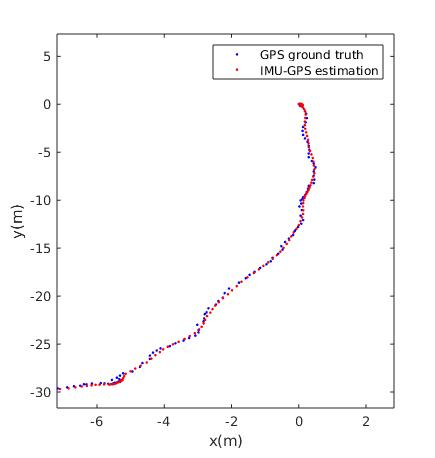
\includegraphics[width = 0.5\linewidth]{media/Starting_results.jpg}
    \caption{Comparison between the IMU-GPS estimation and GPS ground truth in the first 20 secs of data collection}
    \label{fig:imugps-20s}
\end{figure}

\begin{figure}[hbt!]
    \centering
    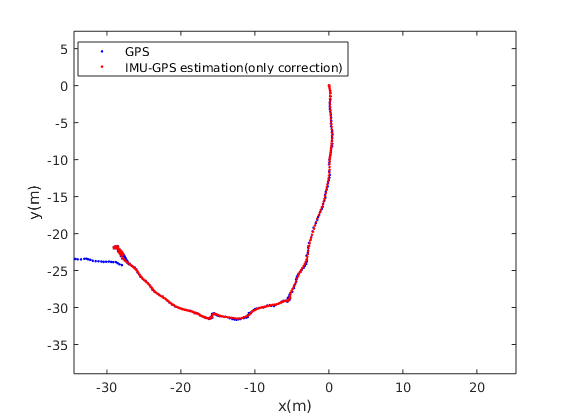
\includegraphics[width = 0.8\linewidth]{media/OnlyGPS.png}
    \caption{Comparison between the filter estimation using only the GPS correction and GPS ground truth in the first 40 secs of data collection}
    \label{fig:imugps-40s}
\end{figure}

Figure \ref{fig:complete_IMUGPS_result} compares the pose estimation from the filter with the ground truth. The starting position of the ground truth is set at the origin.

\begin{figure}[hbt!]
    \centering
    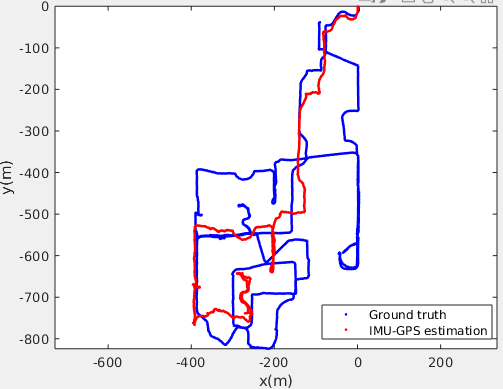
\includegraphics[width = 0.8\linewidth]{media/Complete_InEKF_Result.png}
    \caption{Comparison between the IMU-GPS estimation and the ground truth. About half of the dataset has been processed by the LI-EKF.}
    \label{fig:complete_IMUGPS_result}
\end{figure}




\section{Results and Discussion}\label{sec:results}
\subsection{Incremental SLAM and Loop Closure}

To evaluate the performance of Cartographer, we ran it using the 2012-11-16 run of the NCLT dataset as input. Plots are of the trajectory from the 11 to 13 minute mark from the start of the dataset. The provided ground truth, odometry, and Cartographer operating in 2D and 3D mode are compared. Note that this section evaluates error over a 2 minute long loop, rather than 20 seconds of operation while turning.

We found that for our dataset, we had to assign a high weight to rotation and translation changes in the optimizer, exactly two orders of magnitude greater than the default settings. Higher weights correspond to increased trust in the prior provided by IMU and odometry measurements, meaning that the result of scan-to-submap matching was more likely to introduce error to the output trajectory than the odometry and IMU priors.

Compared to the trajectory smoothing and InEKF approaches, Cartographer's scan-to-submap matching accumulates an order of magnitude less error over 2 minutes than the incremental methods accumulate over 20 seconds. See Table \ref{tb:cartographer-3d-error-table}, Table \ref{tb:cartographer-2d-error-table}, and Table \ref{tb:Error_Table}. However, there is a significant amount of z-axis drift introduced when running Cartographer in 3D mode. This drift is corrected by global optimization at the 56 and 84 second marks, but z-axis error continues to accumulate at about 2 meters per minute. This can be partially remedied by locking the roll and pitch during scan matching, which we have done, but without another method of minimizing z-axis error, it will accumulate enough to prevent larger loops from being closed. Alternatively, additional sensors can be integrated into the optimization problem to correct z-axis error. The Segway also includes data from two Hokuyo lidars, one mounted in a push-broom configuration facing the ground and the other mounted facing forward. The ground-facing lidar could be incorporated into the scan matching algorithm so that tracking the ground is incorporated into the algorithm. Finally, altitude estimates could be integrated from one of the GPS receivers as fixed-frame reference points.

While 2D mode was not prone to accumulating z-axis drift like 3D mode, it was significantly more likely to experience runtime errors (segfaults and assertion failures). Most of Cartographer's development has been focused on optimizing for the 3D use-case, so it's likely that these bugs have gone unnoticed because most applications use the 3D trajectory builder interface.

\begin{table}[h]
	\captionsetup[table]{position=here}
    \caption{\label{tb:cartographer-3d-error-table}
    3D Error Analysis using Cartographer
    }
    \begin{center}
    \resizebox{\linewidth}{!}{
        \begin{tabular}{c | *2{c}}
			\toprule
            Dataset & Mean 3D Pose Error (m) & End 3D Pose Error (m) \\
            \hline
             Odometry Only & 1.09 & 1.73 \\
             Cartographer 3D & 3.16 & 7.34 \\
             Cartographer 2D & 1.87 & 4.97 \\
			\bottomrule
        \end{tabular}}
    \end{center}
\end{table}

\begin{table}[h]
	\captionsetup[table]{position=here}
    \caption{\label{tb:cartographer-2d-error-table}
    2D Error Analysis using Cartographer
    }
    \begin{center}
    \resizebox{\linewidth}{!}{
        \begin{tabular}{c | *2{c}}
			\toprule
            Dataset & Mean 2D Pose Error (m) & End 2D Pose Error (m) \\
            \hline
             Odometry Only & 1.06 & 1.69 \\
             Cartographer 3D & 2.02 & 5.89 \\
             Cartographer 2D & 1.85 & 4.96 \\
			\bottomrule
        \end{tabular}}
    \end{center}
\end{table}

\begin{figure}[hbt!]
    \centering
    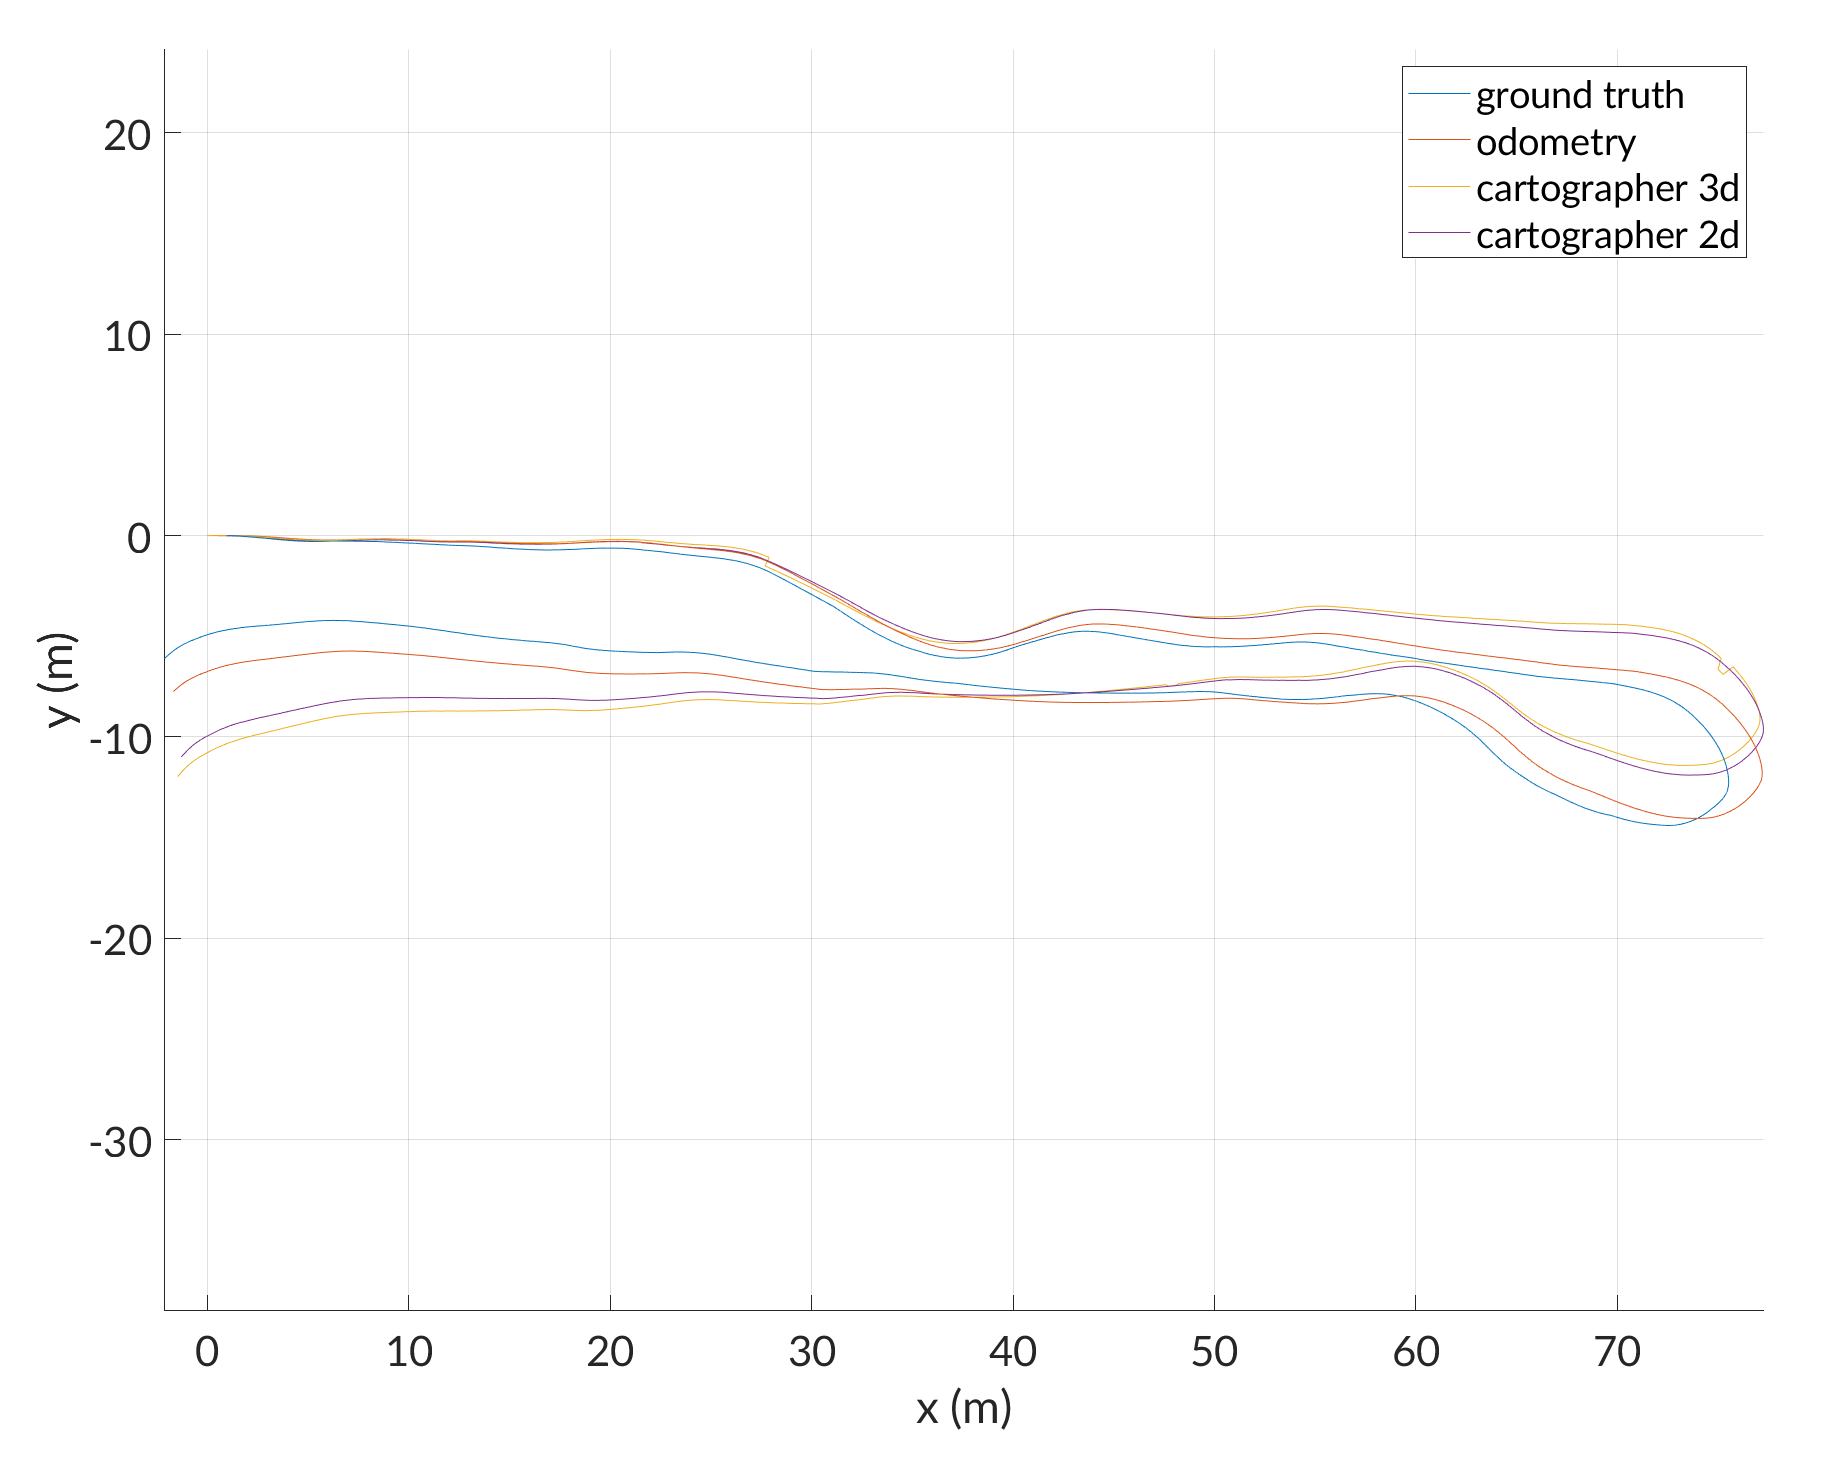
\includegraphics[width = 0.8\linewidth]{media/cartographer/error-top.png}
    \caption{\textit{x-y view of optimized trajectories.}}
    \label{fig:cartographer-xy}
\end{figure}

\begin{figure}[hbt!]
    \centering
    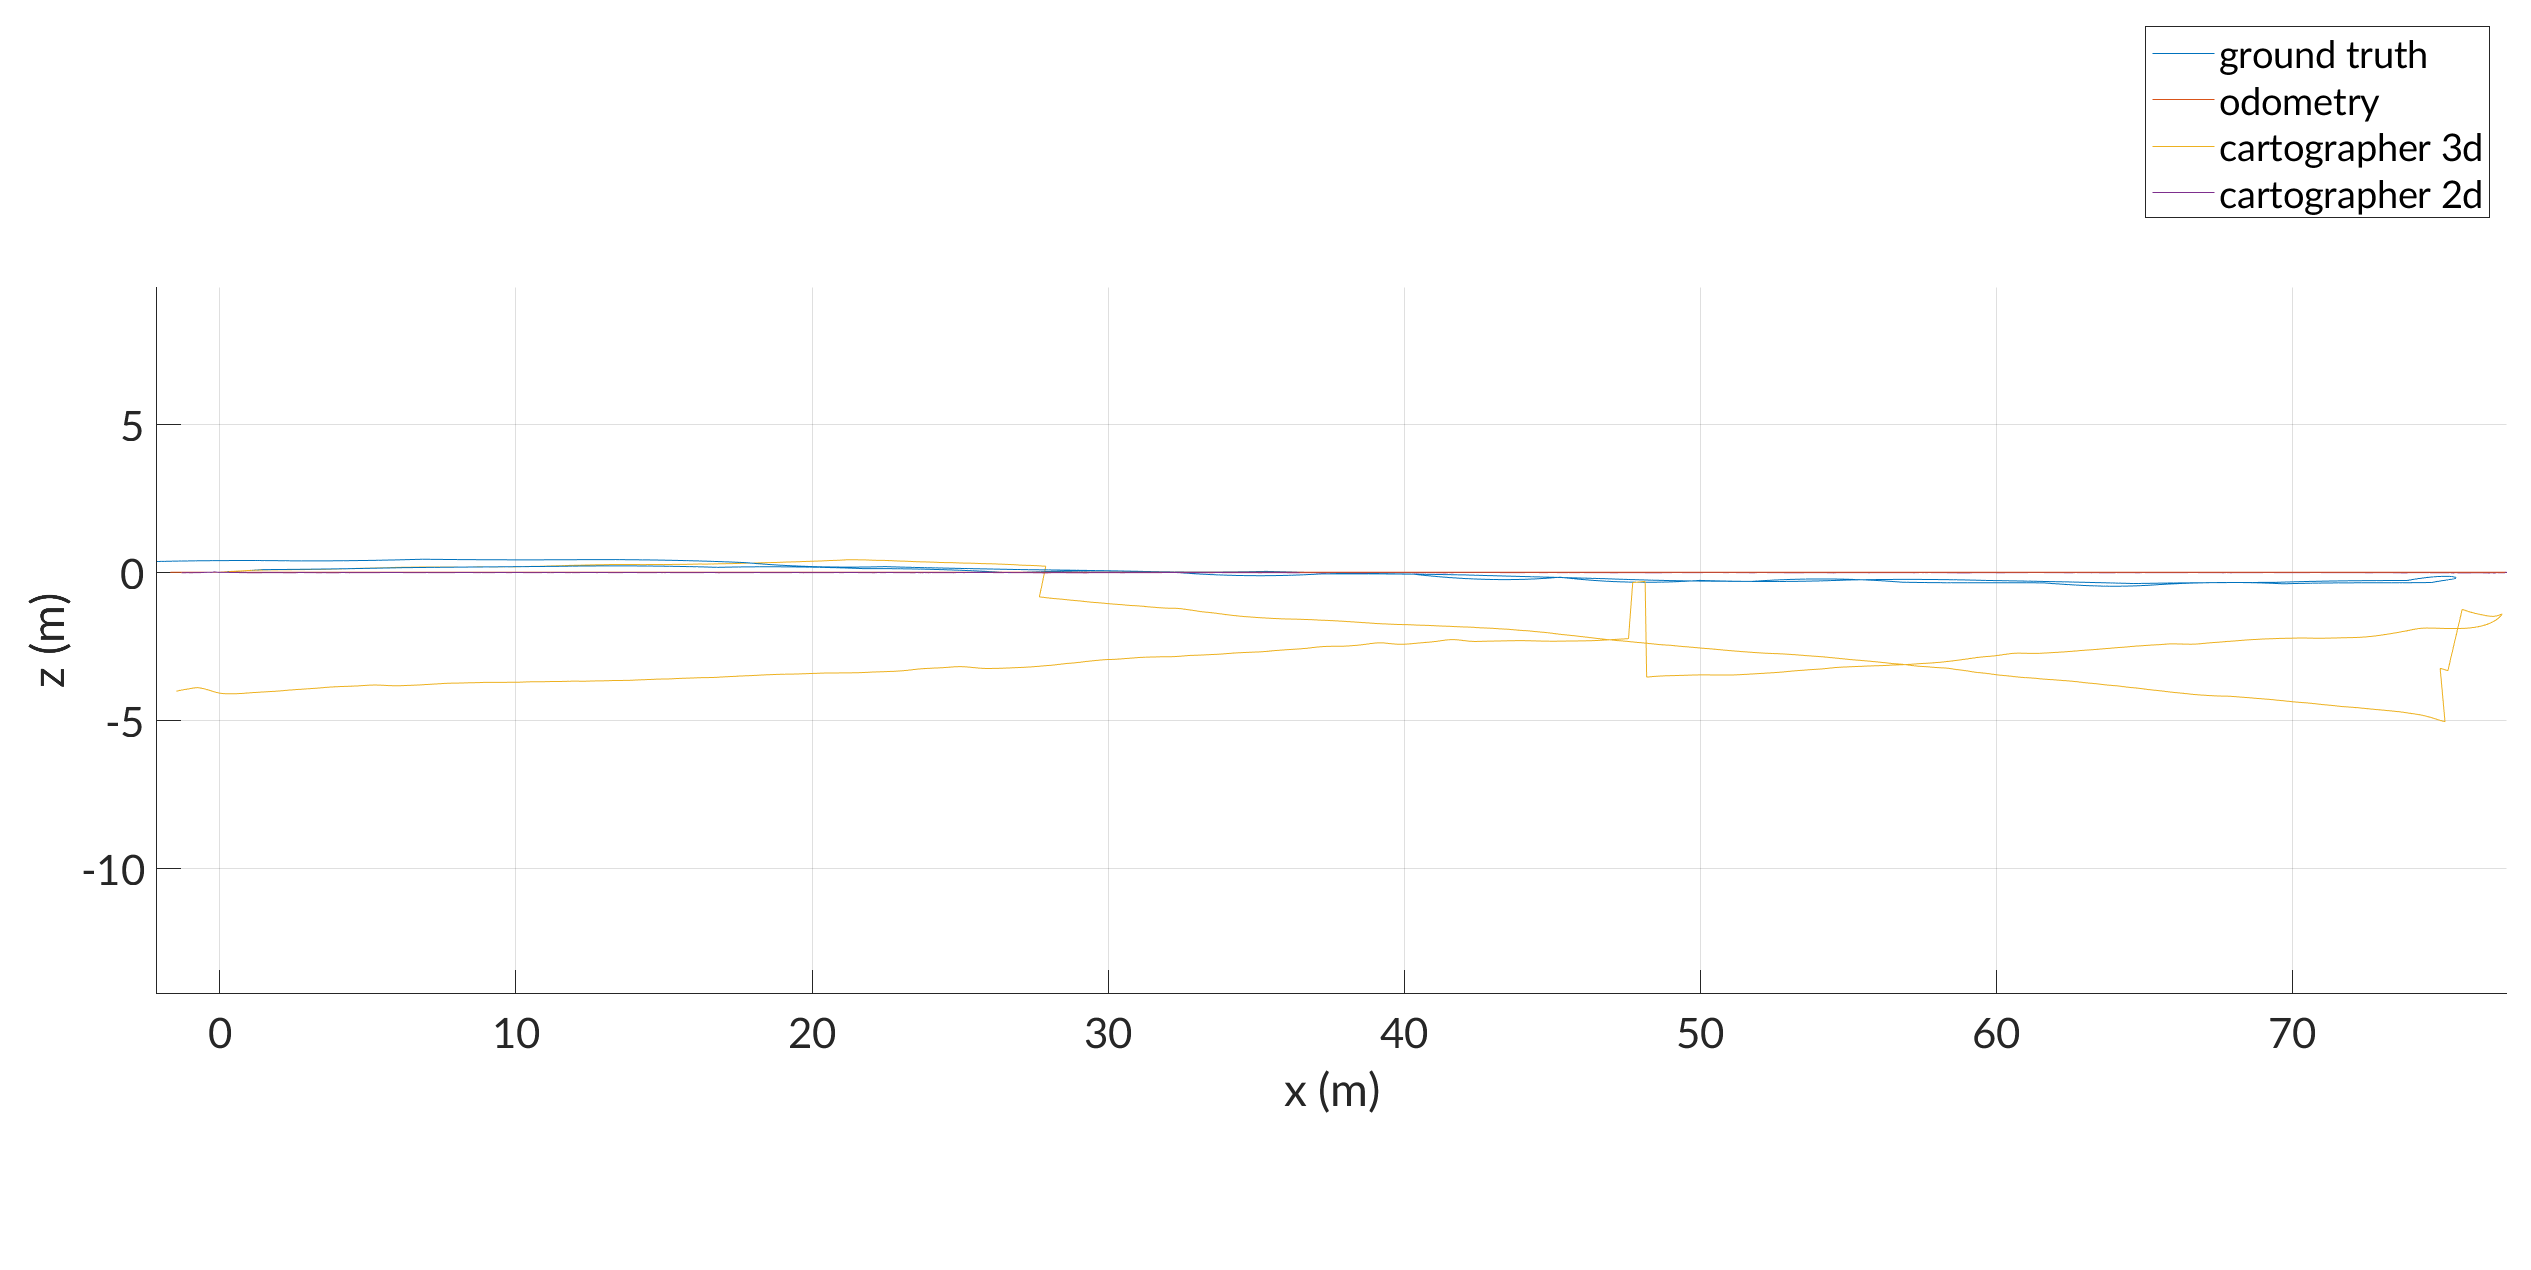
\includegraphics[width = 0.8\linewidth]{media/cartographer/error-side.png}
    \caption{\textit{x-z view of optimized trajectories.}}
    \label{fig:cartographer-xz}
\end{figure}

\begin{figure}[hbt!]
    \centering
    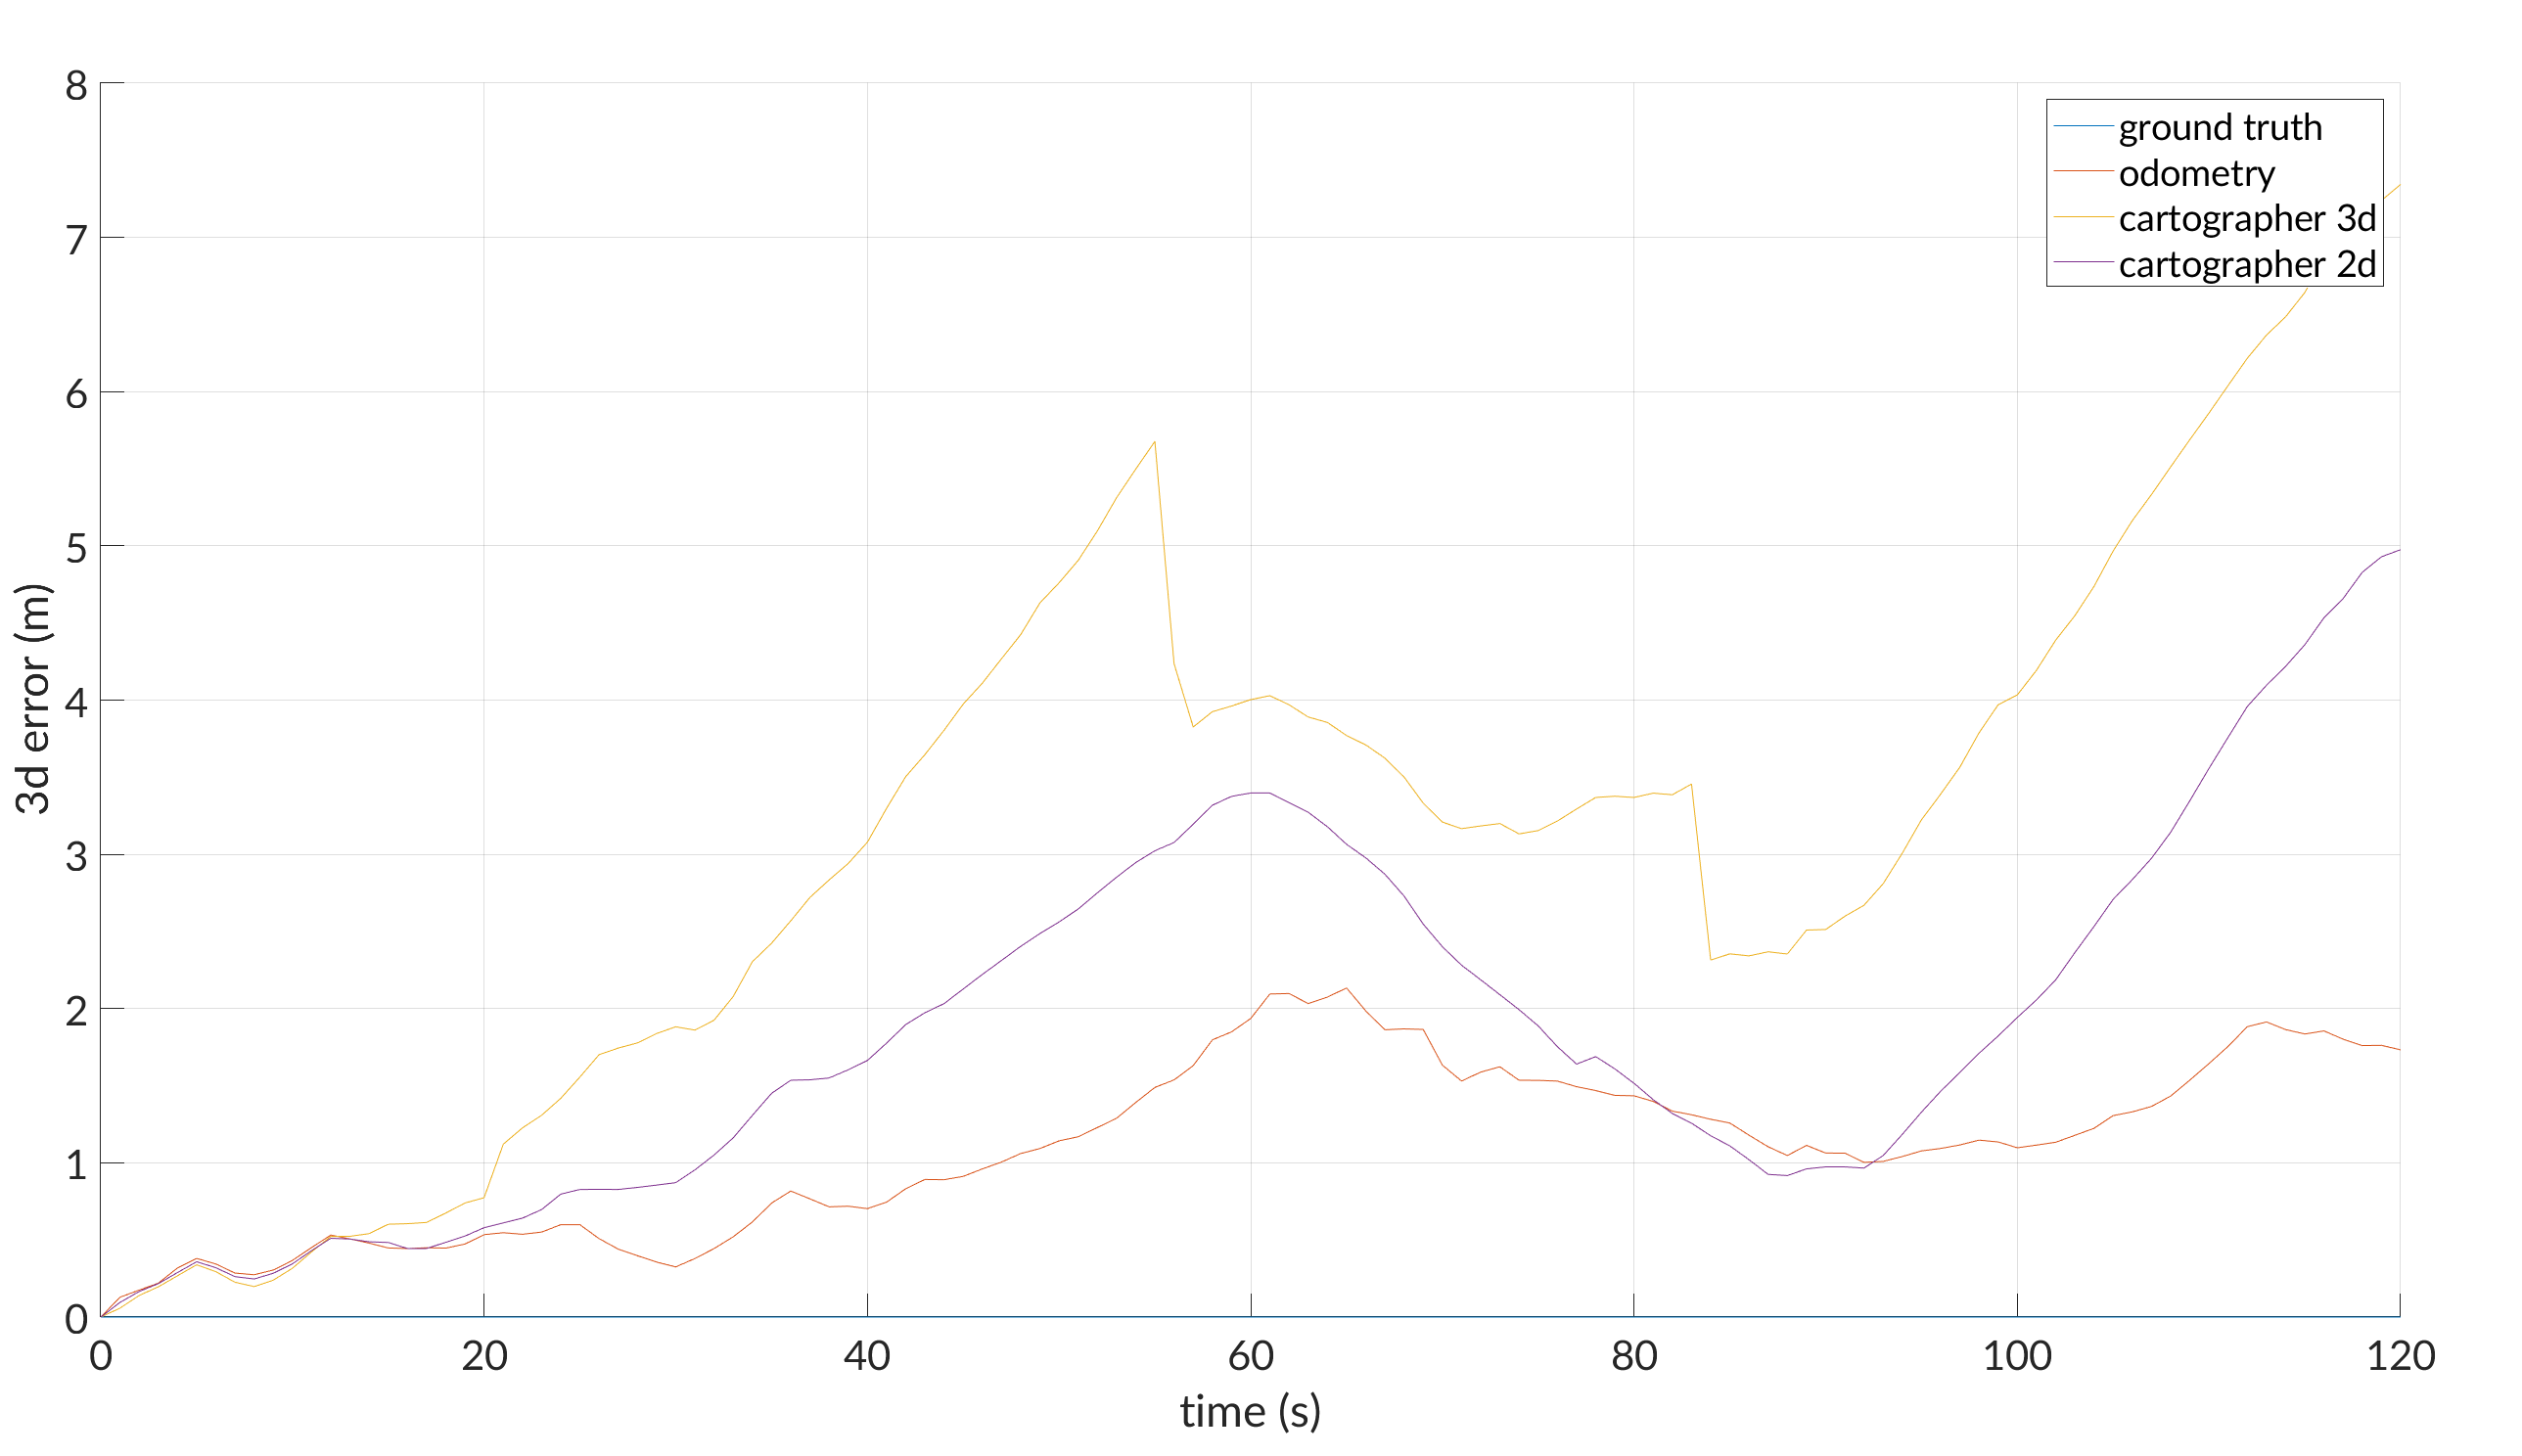
\includegraphics[width = 0.8\linewidth]{media/cartographer/3d-translation-error.png}
    \caption{\textit{3D translation error.}}
    \label{fig:cartographer-3d-error}
\end{figure}

\begin{figure}[hbt!]
    \centering
    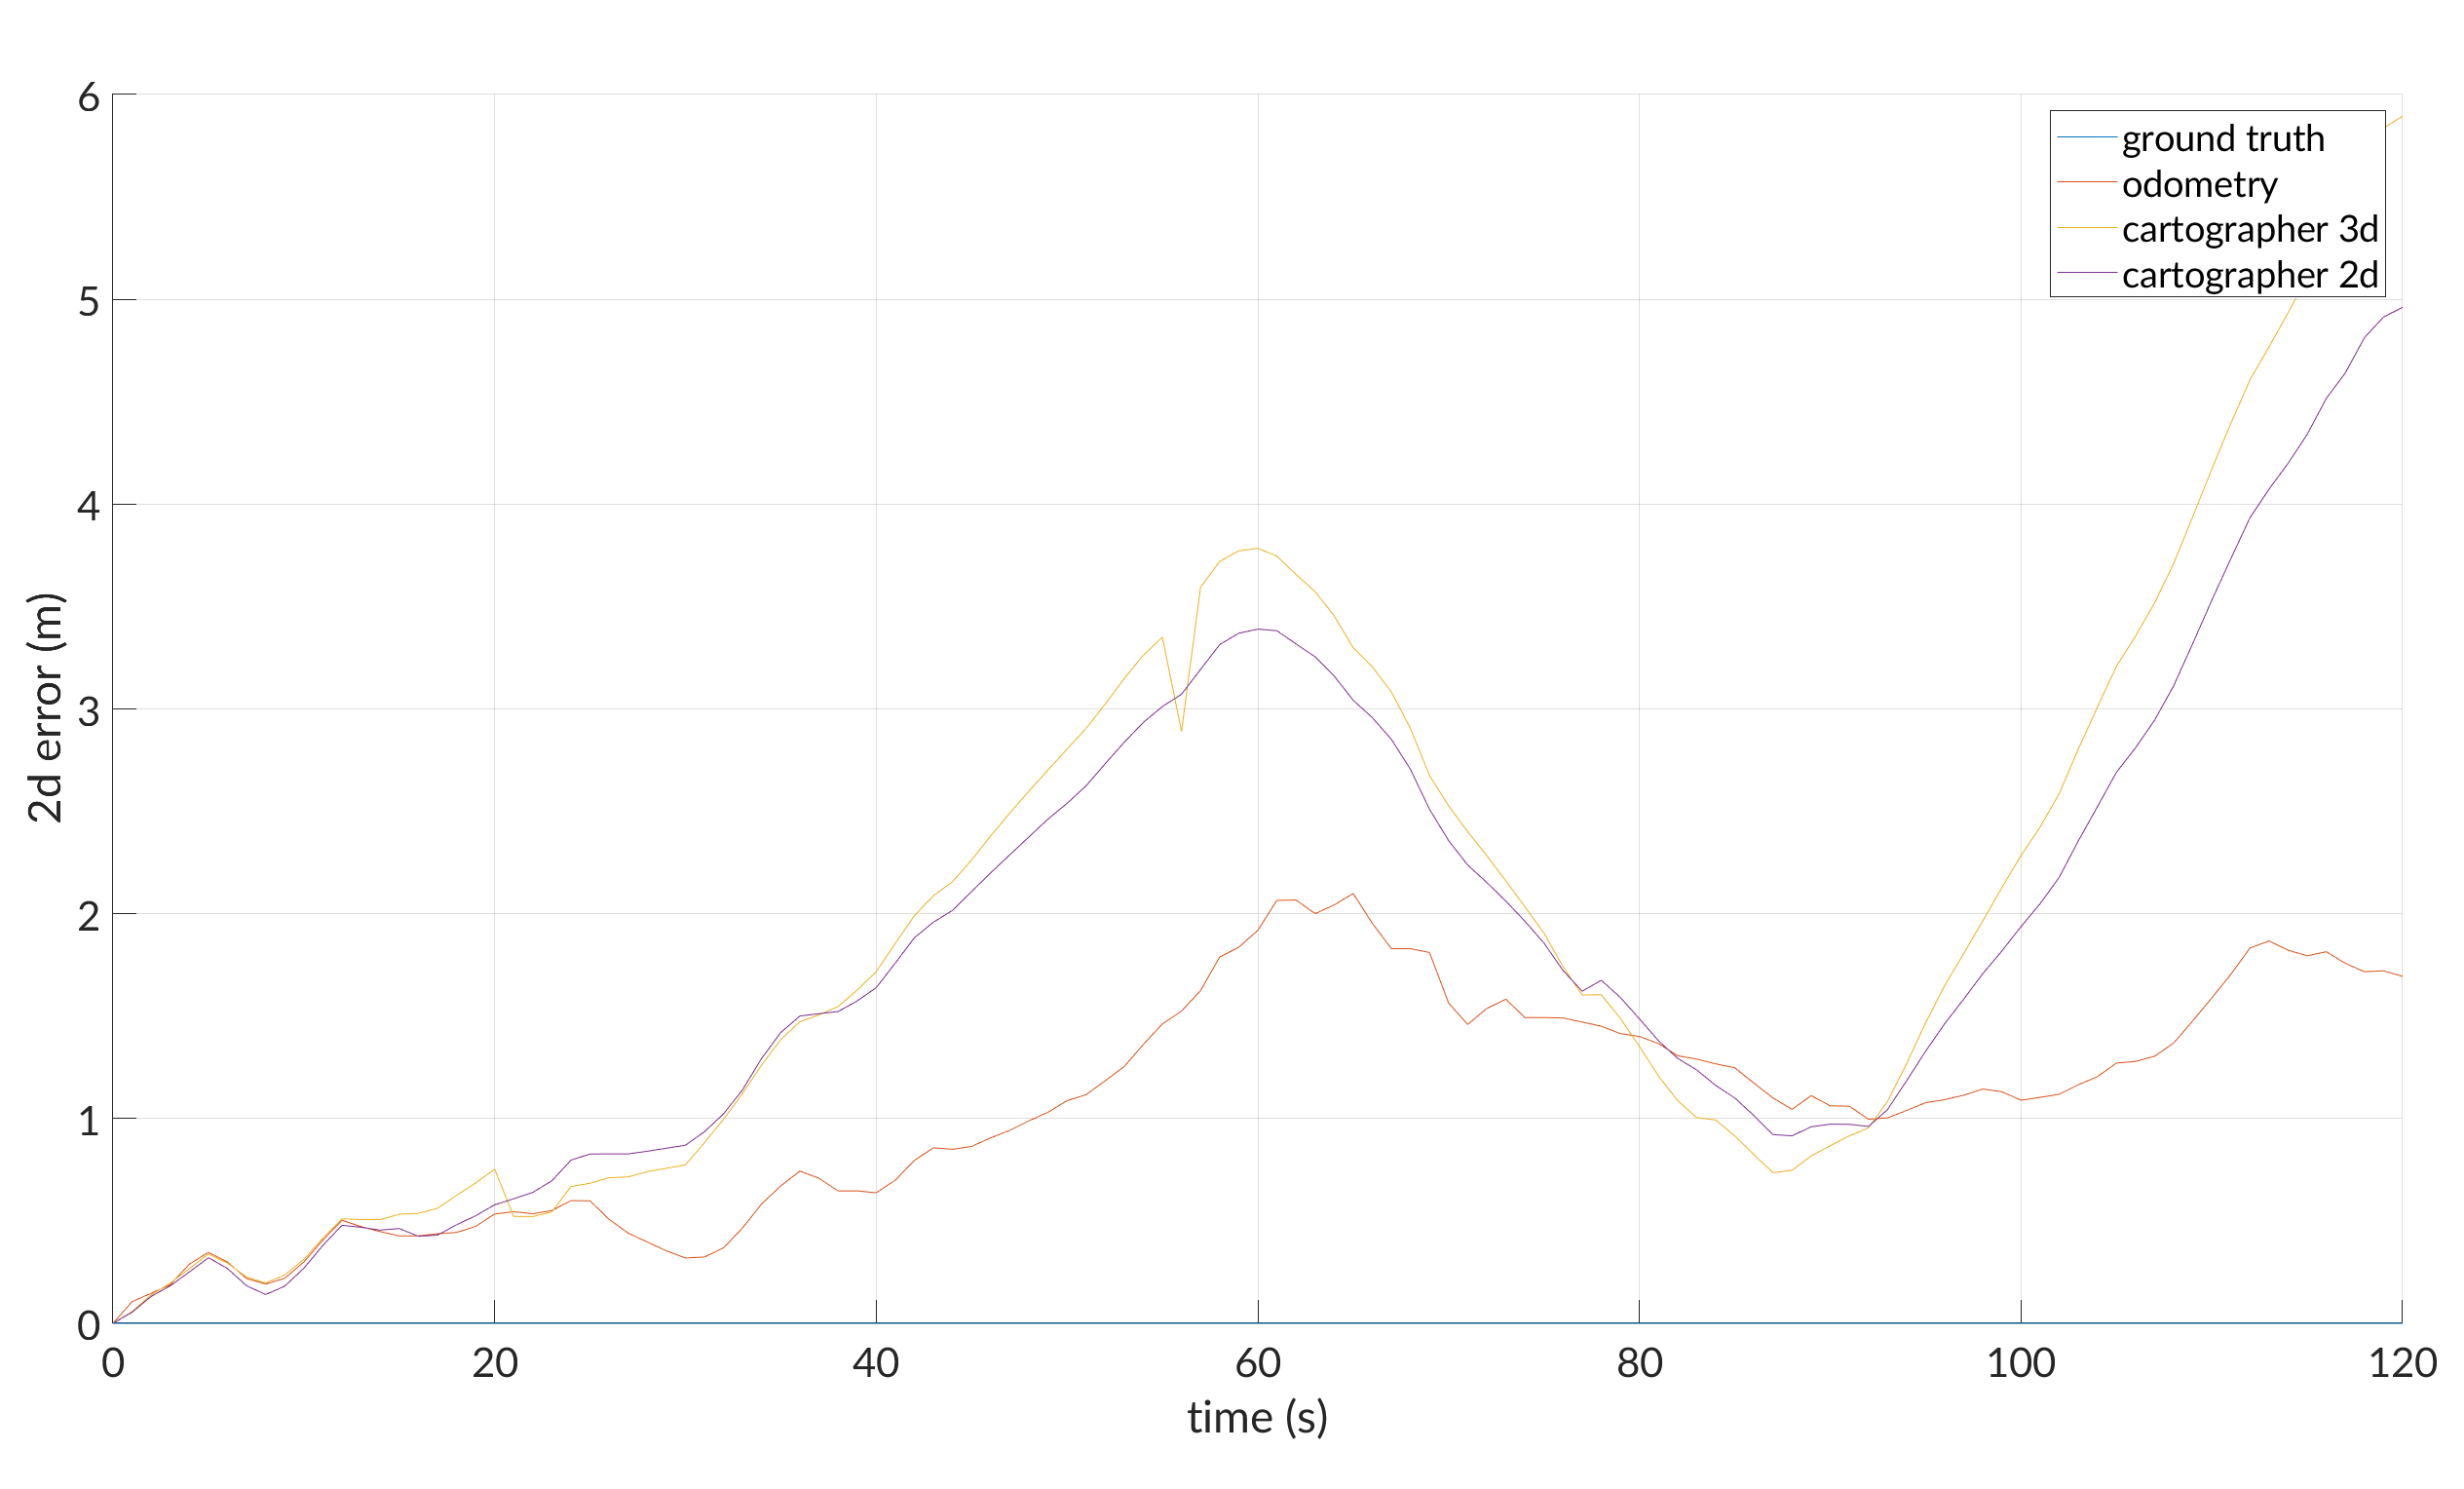
\includegraphics[width = 0.8\linewidth]{media/cartographer/2d-translation-error.png}
    \caption{\textit{2D translation error.}}
    \label{fig:cartographer-2d-error}
\end{figure}

\subsection{Trajectory Smoothing Analysis}
This section includes the error analysis of trajectory smoothing. The main concentration is on mean error,  end pose error and covariance. Mean error in Table. \ref{tb:Error_Table} represents average mean error in meter at each individual step. End pose error refers to the distance error which is equal to $location_{real}(x,y) - location_{ground truth}(x,y)$ Covariance is the covariance between ground truth position and the estimated position. The detail is given in Table. \ref{tb:Error_Table}.

\begin{table}[h]
	\captionsetup[table]{position=here}
    \caption{\label{tb:Error_Table}
    Error Analysis using Trajectory smoothing
    } 
    \begin{center}
    \resizebox{\linewidth}{!}{
        \begin{tabular}{c | *3{c}}
			\toprule
            Dataset & Mean Error(m) & Average Covariance(m\textsuperscript{2}) & End Pose Error(m) \\
            \hline
             $Odometry+Gyro$ & 116.43 & 13783.43 & 154.53  \\
             $Gyrodometry$ & 125.75 & 16482.48 & 178.49 \\
             $GPS+IMU$ & 21.41 & 459.02 &79.94 \\
             $GPS+Odometry$ & 9.14 & 92.41 & 75.95 \\
			\bottomrule
        \end{tabular}}
    \end{center}
\end{table}

\subsubsection{Analysis about odometry Data}
Theoretically, gyrodometry should perform better result than pure odometry and odometry + Gyro data. However, Table.\ref{tb:Error_Table} and Figure.\ref{fig:Gyrodometry} show that ``gyro-only" correction methods beats other odometry correction methods. One of the explanation is that the gyro sensor(KVH DSP-3000 single-axis FOG) in NCLT dataset provides highly accurate rotation measurements. Moreover, the gyro data  biased towards the same side as the odometry data, thus gyro cannot aid the correction of the trajectory a lot.

Additionally, even though the shape of the trajectory looks similar to the ground truth, the error accumulates through the entire trajectory, because there is no sensor measurement for correction. Thus, simply using odometry + Gyro data is not ideal method. The next section brings GPS data into discussion for minimizing the bias of the trajectory. 

\subsubsection{Analysis about GPS Data}
From Figure. \ref{fig:IMU-GPS}, as the GPS data obtained is noisy, lots of overshoots exist in the trajectory. To correct the overshot portion of the trajectory, GPS is preferred to be filtered with IMU data. 

With ISAM2 method, the overshoots can be minimized and filter GPS trajectory can be viewed in Figure. \ref{fig:filteredgps}. To tune a better trajectory, IMU variance value is to set high($\sigma_{angular}$ = 10) on angular direction. Although the filtered GPS trajectory seems to be closer to the ground truth from Table. \ref{tb:Error_Table} and the orientation of the trajectory is about to align with the ground truth, the details of the trajectory is not good enough as the trajectory estimation. Then, to further corrects the trajectory, combing with corrected odometry data would be preferred. 

\subsubsection{Analysis about GPS + Odometry Data}
The filtered Odometry data are used to create graph and filted GPS data are added as factors such that by tuning the covariance values, the trajectory can be further optimized and obtained in Figure. \ref{fig:Final plot}. The strategy to tune a better trajectory is to set sigma large($\sigma_{linear}$ = 100) on linear direction and set low sigma value ($\sigma_{angular}$ = 0.3) on angular direction.

Overall, the filtered data using modified odometry and modified GPS shows the best result among all method in Table. \ref{tb:Error_Table}. However, the filtered trajectory looks bad when the robot drives in a complicated manner shown in Figure \ref{fig:Final plot} (the details of the trajectory is messy). In contrast, the overall filtered trajectory is a good represent of the location of robot when it moves in a relatively simple minor, like driving in a straight line or doing some square movement. One of the possible reason is that the GPS is noisy when the robot performs continuous turning in a short amount of time such that the GPS data cannot be updated correctly.

% To do: edit the latex structure

\subsection{Left-InEKF Analysis}

This section examines the result from the Left-InEKF. By comparing the result with the given ground truth, error analysis is performed and presented in Table \ref{tb:Error_Table_2}.

\begin{table}[h]
	\captionsetup[table]{position=here}
    \caption{\label{tb:Error_Table_2}
    Error Analysis for Left-InEKF
    } 
    \begin{center}
    \resizebox{\linewidth}{!}{
        \begin{tabular}{c | *3{c}}
			\toprule
            Dataset & Mean Error(m) & Average Covariance(m\textsuperscript{2}) & End Pose Error(m) \\
            \hline
             $GPS+IMU InEKF$ & 95.32 & 8801.55 &109.94 \\
			\bottomrule
        \end{tabular}}
    \end{center}
\end{table}

In comparison with the trajectory smoothing output using GPS and IMU (Table \ref{tb:Error_Table}), the InEKF estimation has approximately 10\% larger error. As shown in Figure \ref{fig:complete_IMUGPS_result}, the estimation is the most accurate at the beginning of the data collection, starting at the origin. However, it gradually deviates away from the ground truth, despite of the general shapes of the two plots being similar. 

The error may have been caused by the following reasons. First, the covariance is not well tuned for the filter. If a larger sigma is assigned to the input and observation, a more accurate estimation will be obtained. Second, the GPS data is rather jumpy as shown in Figure \ref{fig:IMU-GPS}. If the GPS measurement is smoothed before inputting into the filter, the result could have been be better. In addition, the overall size of the estimated trajectory is larger than that of the ground truth, which indicates a probable system error in the calculation to transform the latitude and longitude to the x-y location. Lastly, when the IMU dataset was re-sampled, a 5\% time difference was generated between the IMU and GPS measurements. The goal of resampling was to ensure a same number of prediction and correction steps in the algorithm. A more complete method is to utilize the full length of the IMU data and only perform the correction when a GPS measurement is made. 

In general, the Left-InEKF produces a better result than the IMU-only or GPS-only position estimation. The filter can be improved by addressing the three issues mentioned above. 



\section{Conclusion}\label{sec:conclusion}
    Data from 5 different sesors were combined in different combination to implement three different trajectory estimation methods. 
    %We implemented and compared three different trajectory estimation methods in this project. 5 different kinds of sensors are included and fused, including odometry, gyroscope, GPS, IMU, and lidar. These data are combined in different ways and implemented in three methods mentioned. 
    From the provided results and the error analysis, all three methods provide an overall satisfactory trajectory. However, the results are not perfect due to the noisy input data which was present even after filtering, as shown in Figure \ref{fig:Final plot} and Figure \ref{fig:complete_IMUGPS_result}, and the three methods have scope for improvement. Thus, the following improvements can be carried out in the future:

\begin{enumerate}
    \item GPS sensor noise should be reduced to avoid jumpy data, 
    \item A z-axis correction method should be added to the incremental SLAM implementation to correct drift
    \item A more accurate method to linearize GPS coordinates to the local x-y plane
\end{enumerate}


\section{Presentation and GitHub Repository}
\link{https://youtu.be/UGMAuZjeV3A}{Video.}  \\
\link{https://github.com/Gregory-Meyer/mobile-robotics-final-project}{GitHub repository.}
\bibliographystyle{IEEEtran}
\bibliography{ref.bib}

\end{document}